\documentclass[]{article}
\usepackage{lmodern}
\usepackage{amssymb,amsmath}
\usepackage{ifxetex,ifluatex}
\usepackage{fixltx2e} % provides \textsubscript
\ifnum 0\ifxetex 1\fi\ifluatex 1\fi=0 % if pdftex
  \usepackage[T1]{fontenc}
  \usepackage[utf8]{inputenc}
\else % if luatex or xelatex
  \ifxetex
    \usepackage{mathspec}
  \else
    \usepackage{fontspec}
  \fi
  \defaultfontfeatures{Ligatures=TeX,Scale=MatchLowercase}
\fi
% use upquote if available, for straight quotes in verbatim environments
\IfFileExists{upquote.sty}{\usepackage{upquote}}{}
% use microtype if available
\IfFileExists{microtype.sty}{%
\usepackage{microtype}
\UseMicrotypeSet[protrusion]{basicmath} % disable protrusion for tt fonts
}{}
\usepackage[margin=1in]{geometry}
\usepackage{hyperref}
\hypersetup{unicode=true,
            pdftitle={nba\_data\_visV5},
            pdfauthor={Justin Huang},
            pdfborder={0 0 0},
            breaklinks=true}
\urlstyle{same}  % don't use monospace font for urls
\usepackage{color}
\usepackage{fancyvrb}
\newcommand{\VerbBar}{|}
\newcommand{\VERB}{\Verb[commandchars=\\\{\}]}
\DefineVerbatimEnvironment{Highlighting}{Verbatim}{commandchars=\\\{\}}
% Add ',fontsize=\small' for more characters per line
\usepackage{framed}
\definecolor{shadecolor}{RGB}{248,248,248}
\newenvironment{Shaded}{\begin{snugshade}}{\end{snugshade}}
\newcommand{\KeywordTok}[1]{\textcolor[rgb]{0.13,0.29,0.53}{\textbf{#1}}}
\newcommand{\DataTypeTok}[1]{\textcolor[rgb]{0.13,0.29,0.53}{#1}}
\newcommand{\DecValTok}[1]{\textcolor[rgb]{0.00,0.00,0.81}{#1}}
\newcommand{\BaseNTok}[1]{\textcolor[rgb]{0.00,0.00,0.81}{#1}}
\newcommand{\FloatTok}[1]{\textcolor[rgb]{0.00,0.00,0.81}{#1}}
\newcommand{\ConstantTok}[1]{\textcolor[rgb]{0.00,0.00,0.00}{#1}}
\newcommand{\CharTok}[1]{\textcolor[rgb]{0.31,0.60,0.02}{#1}}
\newcommand{\SpecialCharTok}[1]{\textcolor[rgb]{0.00,0.00,0.00}{#1}}
\newcommand{\StringTok}[1]{\textcolor[rgb]{0.31,0.60,0.02}{#1}}
\newcommand{\VerbatimStringTok}[1]{\textcolor[rgb]{0.31,0.60,0.02}{#1}}
\newcommand{\SpecialStringTok}[1]{\textcolor[rgb]{0.31,0.60,0.02}{#1}}
\newcommand{\ImportTok}[1]{#1}
\newcommand{\CommentTok}[1]{\textcolor[rgb]{0.56,0.35,0.01}{\textit{#1}}}
\newcommand{\DocumentationTok}[1]{\textcolor[rgb]{0.56,0.35,0.01}{\textbf{\textit{#1}}}}
\newcommand{\AnnotationTok}[1]{\textcolor[rgb]{0.56,0.35,0.01}{\textbf{\textit{#1}}}}
\newcommand{\CommentVarTok}[1]{\textcolor[rgb]{0.56,0.35,0.01}{\textbf{\textit{#1}}}}
\newcommand{\OtherTok}[1]{\textcolor[rgb]{0.56,0.35,0.01}{#1}}
\newcommand{\FunctionTok}[1]{\textcolor[rgb]{0.00,0.00,0.00}{#1}}
\newcommand{\VariableTok}[1]{\textcolor[rgb]{0.00,0.00,0.00}{#1}}
\newcommand{\ControlFlowTok}[1]{\textcolor[rgb]{0.13,0.29,0.53}{\textbf{#1}}}
\newcommand{\OperatorTok}[1]{\textcolor[rgb]{0.81,0.36,0.00}{\textbf{#1}}}
\newcommand{\BuiltInTok}[1]{#1}
\newcommand{\ExtensionTok}[1]{#1}
\newcommand{\PreprocessorTok}[1]{\textcolor[rgb]{0.56,0.35,0.01}{\textit{#1}}}
\newcommand{\AttributeTok}[1]{\textcolor[rgb]{0.77,0.63,0.00}{#1}}
\newcommand{\RegionMarkerTok}[1]{#1}
\newcommand{\InformationTok}[1]{\textcolor[rgb]{0.56,0.35,0.01}{\textbf{\textit{#1}}}}
\newcommand{\WarningTok}[1]{\textcolor[rgb]{0.56,0.35,0.01}{\textbf{\textit{#1}}}}
\newcommand{\AlertTok}[1]{\textcolor[rgb]{0.94,0.16,0.16}{#1}}
\newcommand{\ErrorTok}[1]{\textcolor[rgb]{0.64,0.00,0.00}{\textbf{#1}}}
\newcommand{\NormalTok}[1]{#1}
\usepackage{graphicx,grffile}
\makeatletter
\def\maxwidth{\ifdim\Gin@nat@width>\linewidth\linewidth\else\Gin@nat@width\fi}
\def\maxheight{\ifdim\Gin@nat@height>\textheight\textheight\else\Gin@nat@height\fi}
\makeatother
% Scale images if necessary, so that they will not overflow the page
% margins by default, and it is still possible to overwrite the defaults
% using explicit options in \includegraphics[width, height, ...]{}
\setkeys{Gin}{width=\maxwidth,height=\maxheight,keepaspectratio}
\IfFileExists{parskip.sty}{%
\usepackage{parskip}
}{% else
\setlength{\parindent}{0pt}
\setlength{\parskip}{6pt plus 2pt minus 1pt}
}
\setlength{\emergencystretch}{3em}  % prevent overfull lines
\providecommand{\tightlist}{%
  \setlength{\itemsep}{0pt}\setlength{\parskip}{0pt}}
\setcounter{secnumdepth}{0}
% Redefines (sub)paragraphs to behave more like sections
\ifx\paragraph\undefined\else
\let\oldparagraph\paragraph
\renewcommand{\paragraph}[1]{\oldparagraph{#1}\mbox{}}
\fi
\ifx\subparagraph\undefined\else
\let\oldsubparagraph\subparagraph
\renewcommand{\subparagraph}[1]{\oldsubparagraph{#1}\mbox{}}
\fi

%%% Use protect on footnotes to avoid problems with footnotes in titles
\let\rmarkdownfootnote\footnote%
\def\footnote{\protect\rmarkdownfootnote}

%%% Change title format to be more compact
\usepackage{titling}

% Create subtitle command for use in maketitle
\newcommand{\subtitle}[1]{
  \posttitle{
    \begin{center}\large#1\end{center}
    }
}

\setlength{\droptitle}{-2em}

  \title{nba\_data\_visV5}
    \pretitle{\vspace{\droptitle}\centering\huge}
  \posttitle{\par}
    \author{Justin Huang}
    \preauthor{\centering\large\emph}
  \postauthor{\par}
      \predate{\centering\large\emph}
  \postdate{\par}
    \date{2019-01-17}


\begin{document}
\maketitle

These were all the libraries used to help with data exploration of the
NBA data set.

\begin{Shaded}
\begin{Highlighting}[]
\KeywordTok{library}\NormalTok{(dplyr)}
\KeywordTok{library}\NormalTok{(ggplot2)}
\KeywordTok{library}\NormalTok{(tidyr)}
\KeywordTok{library}\NormalTok{(stringr)}
\KeywordTok{library}\NormalTok{(data.table)}
\KeywordTok{library}\NormalTok{(ggrepel)}
\KeywordTok{library}\NormalTok{(directlabels)}
\KeywordTok{library}\NormalTok{(gridExtra)}
\KeywordTok{options}\NormalTok{(}\DataTypeTok{max.print =} \DecValTok{999999999}\NormalTok{)}
\KeywordTok{options}\NormalTok{(}\DataTypeTok{scipen=}\DecValTok{12}\NormalTok{)}
\end{Highlighting}
\end{Shaded}

\begin{verbatim}
## [1] "/Users/justinvhuang/Desktop/nba_stat_salaries"
\end{verbatim}

\begin{verbatim}
## [1] "/Users/justinvhuang/Desktop/nba_stat_salaries"
\end{verbatim}

\subsubsection{Live and Die by the
Three}\label{live-and-die-by-the-three}

The first thing that we should explore as a NBA team looking to have a
succesful season in the modern era is to see the increased number of 3
point shots. How the NBA team according to many news articles has
evolved into a spacing oriented and 3 point focused game during the
regular season.

\begin{itemize}
\tightlist
\item
  {[}3 Point
  Revolution{]}\{\url{https://www.cbssports.com/nba/news/whats-the-end-game-for-nbas-3-point-revolution-coaches-and-players-sound-off-on-the-games-most-dominant-shot/}\}
\item
  {[}More 3's the
  Better{]}\{\url{https://www.deseretnews.com/article/900019954/why-the-3-point-shot-has-become-too-much-of-a-good-thing.html}\}
\item
  {[}Warriors and the
  3's{]}\{\url{https://sports.yahoo.com/warriors-fall-behind-nba-3-172136589.html}\}
\end{itemize}

Let us first look at the distrubtion of the 3 point shot made, 2 point
shot made and salary.

\begin{verbatim}
##   median(salary) mean(salary) sd(salary)    var(salary) IQR(salary)
## 1        2678400      4523495    4862128 23640286672352     4899590
\end{verbatim}

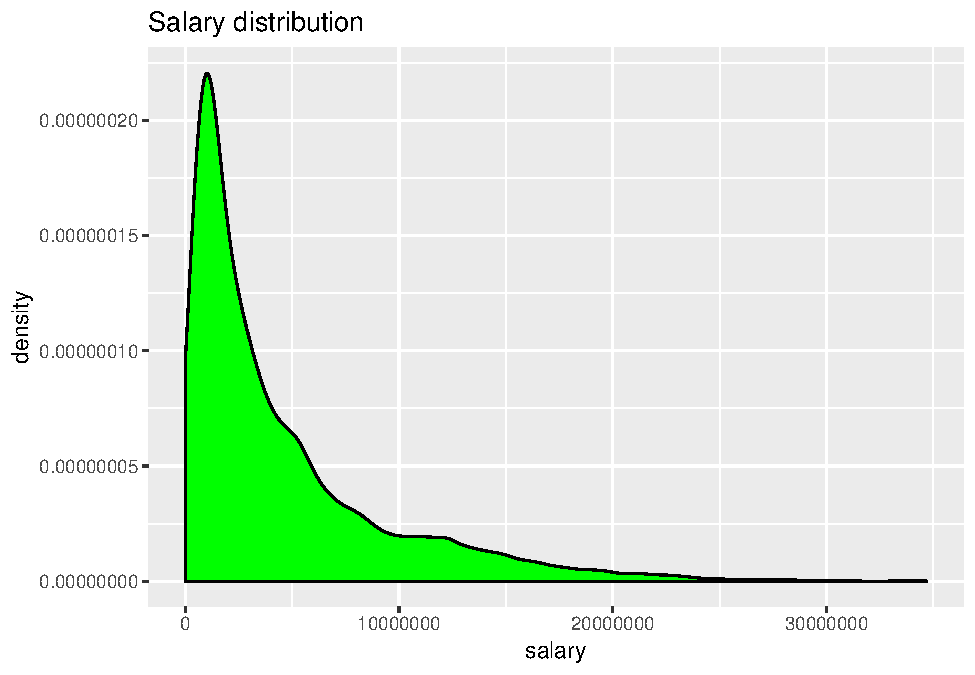
\includegraphics{nba_data_visV4_files/figure-latex/unnamed-chunk-3-1.pdf}

There seems to be a right skew in the data. Showing that superstars and
stars get the biggest pay day and take the biggest proportion of the
teams salary.

\begin{verbatim}
##   median(two) mean(two)  sd(two) var(two) IQR(two)
## 1         2.1  2.667674 1.899015  3.60626      2.5
\end{verbatim}

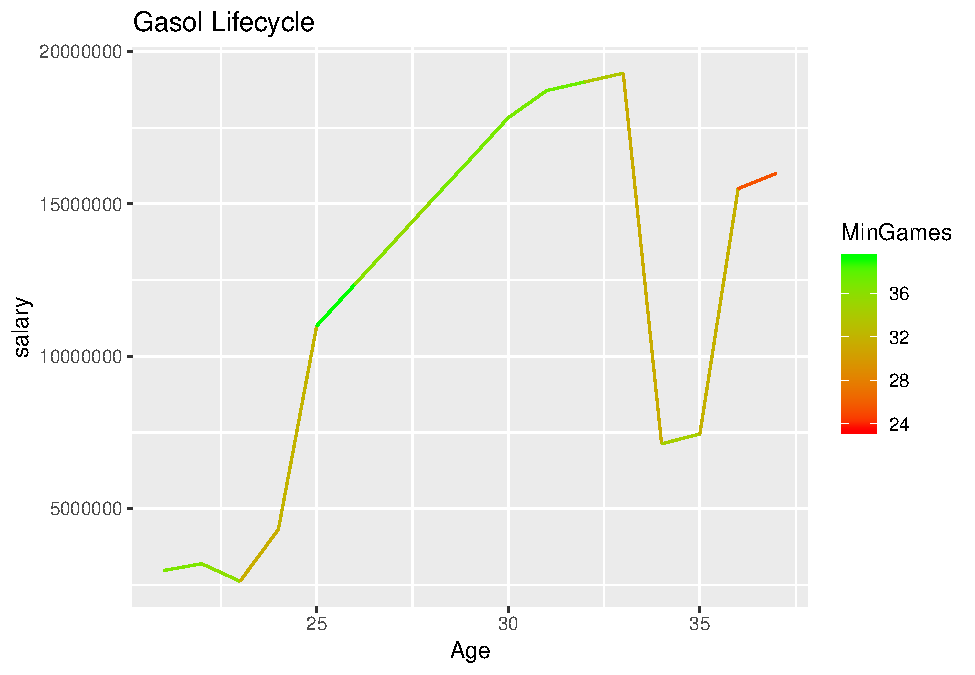
\includegraphics{nba_data_visV4_files/figure-latex/unnamed-chunk-4-1.pdf}

\begin{verbatim}
##   median(three) mean(three) sd(three) var(three) IQR(three)
## 1           0.3   0.5867761 0.6674279  0.4454601          1
\end{verbatim}

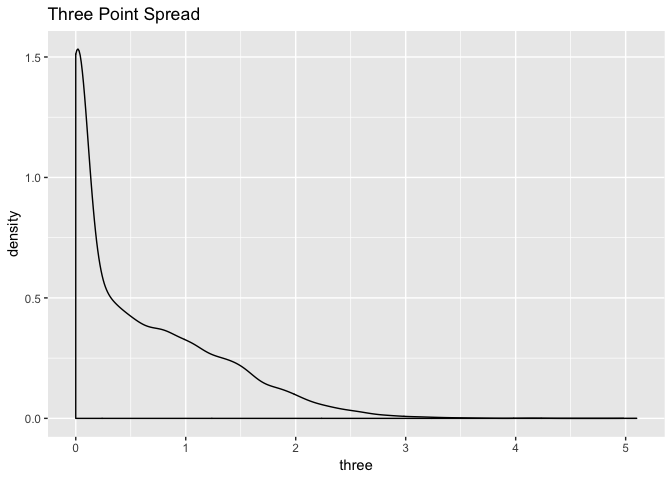
\includegraphics{nba_data_visV4_files/figure-latex/unnamed-chunk-4-2.pdf}

Both are right skewed showing that the stars and main players on the
team usually take most of the shots.

Lets now look at the trend over the years of the three point shot vs two
point shot.

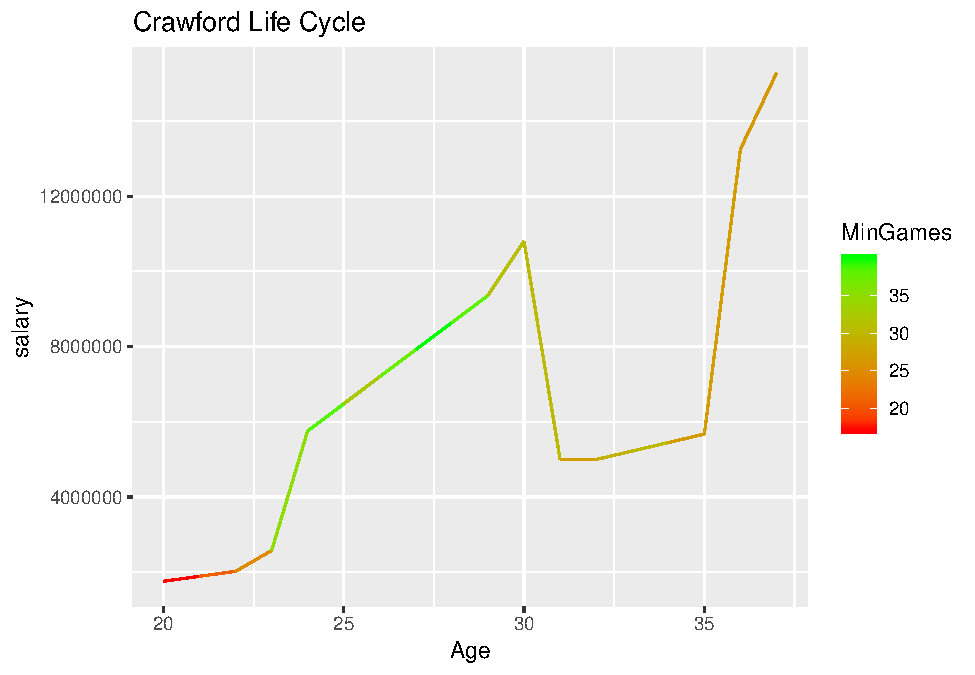
\includegraphics{nba_data_visV4_files/figure-latex/unnamed-chunk-5-1.pdf}

The mean 3 point shots have been increasing indicated by the trending
upward blue dots. While the number of 2 point shots have been decreasing
by the red dots going down.

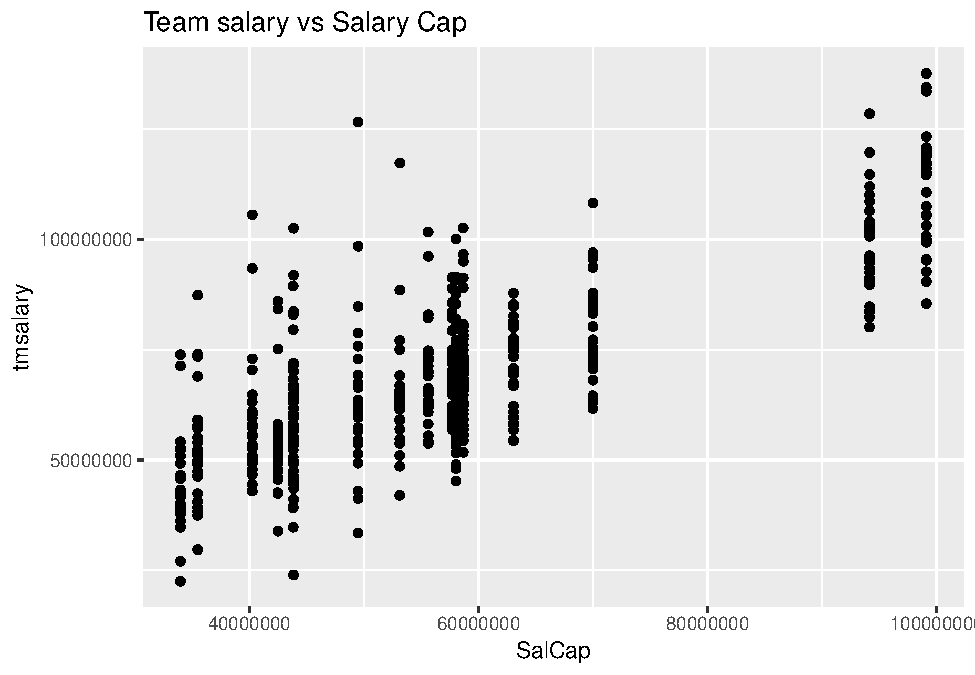
\includegraphics{nba_data_visV4_files/figure-latex/unnamed-chunk-6-1.pdf}

For players who took more than three 3's a game there is an increase in
salary after the 2015 year. However, there is still a decrease before
then. Perhaps teams didn't pay big salaries for 3 point specialist
earlier on and emphasized on other basketball statistics.

Let us explore if 3 pointers lead to more wins

\includegraphics{nba_data_visV4_files/figure-latex/unnamed-chunk-7-1.pdf}

2014 seems to be an increase in wins for taking more than three 3's a
game. Before that the league was more big man focused with players such
as Kevin Garnett, Tim Duncan, Shaquille O'neal, Jermaine O'neal, Dwight
Howard.

Now let us explore the other end of the spectrum. With less than three
3's a game.

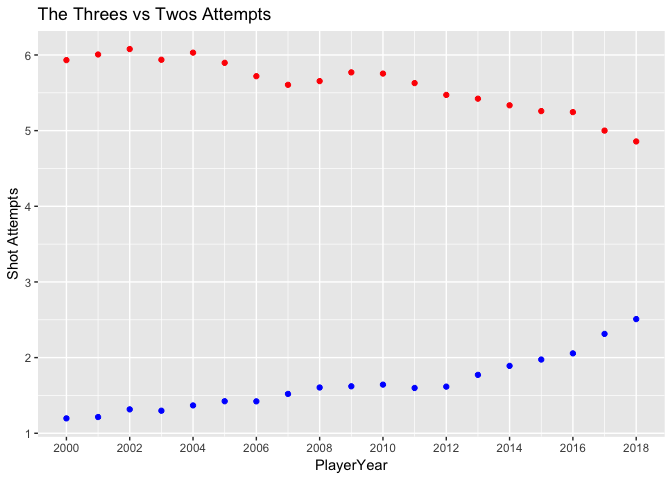
\includegraphics{nba_data_visV4_files/figure-latex/unnamed-chunk-8-1.pdf}

There is still an increase in salary. This is due to the TV contract
money with the NBA increasing the salary cap which was a huge factor.
However, if you look at the summary of the mins and max you can see
taking more than 3 threes a game is beneficial.

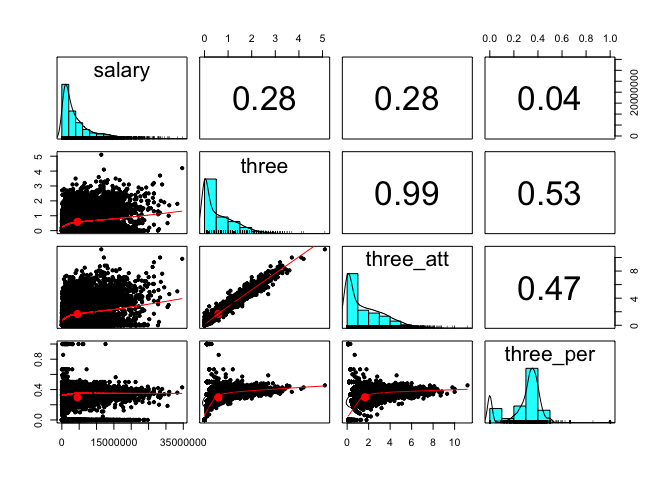
\includegraphics{nba_data_visV4_files/figure-latex/unnamed-chunk-9-1.pdf}

Attemping more 3's is benefical it looks like. From the years 2004 to
2008 the league still had traditional big men who dominated the league.
Spacing and rules didn't emphasize spacing as much. Having players that
take less than three 3's a game leads to a team win that would be 8th
seed in the east and out of the playoffs in the western conference.

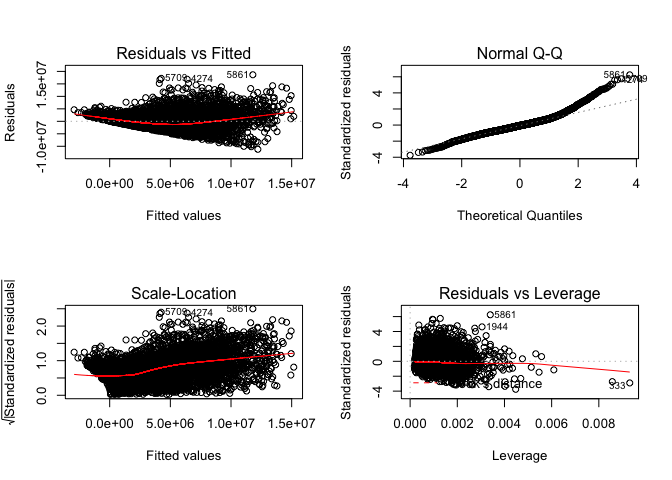
\includegraphics{nba_data_visV4_files/figure-latex/unnamed-chunk-10-1.pdf}

Making more two's of course leads to a better salary. The TV money seems
have a major factor to increase the salary for the players after 2015.

Conclusion:

Overall 3 point shooting does lead to more wins and an increase of
salary. However, due to the TV contract there was a huge salary bump as
well as new CBA and talks with the players association.

\subsubsection{PPG vs EFG}\label{ppg-vs-efg}

With the increased reliance on data interpretation what we want to
explore is the rise of EFG vs PPG. Players like Rudy Gay and Josh Smith
who scored in bunches before used to be rewarded huge contracts.
However, it was later found they scored inefficiently.

\[ EFG = (FG + 0.5 * 3P) / FGA. \]

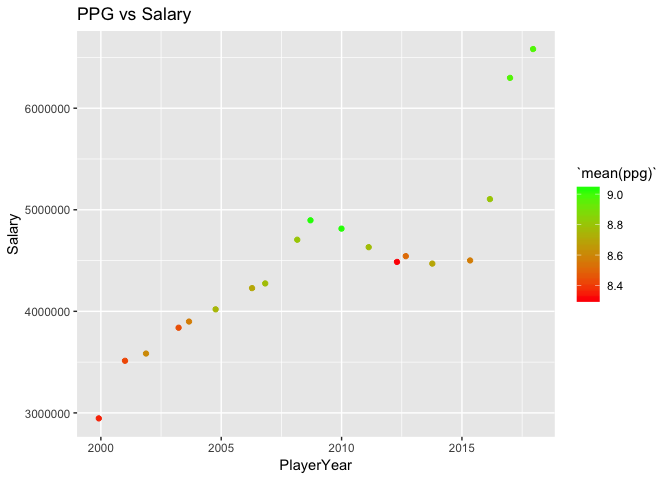
\includegraphics{nba_data_visV4_files/figure-latex/unnamed-chunk-11-1.pdf}

Salary over the years has increased. But there doesn't seem to be a
clear relationship with points per game over the years and salary.

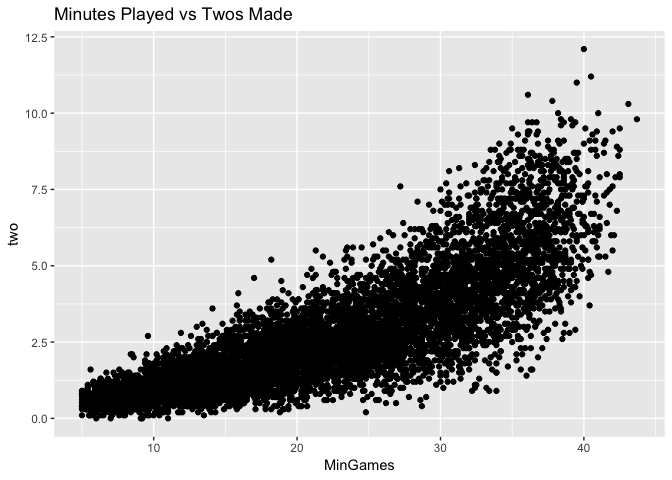
\includegraphics{nba_data_visV4_files/figure-latex/unnamed-chunk-12-1.pdf}

EFG seems to be trending in the later years. As more GMs and teams look
at data they are paying more for players who are shooting more
effectively. In the past teams perhaps were only looking at points per
game.

Lets look at a 20 ppg scorer vs a 50 percent EFG players and see how
their salaries compare.

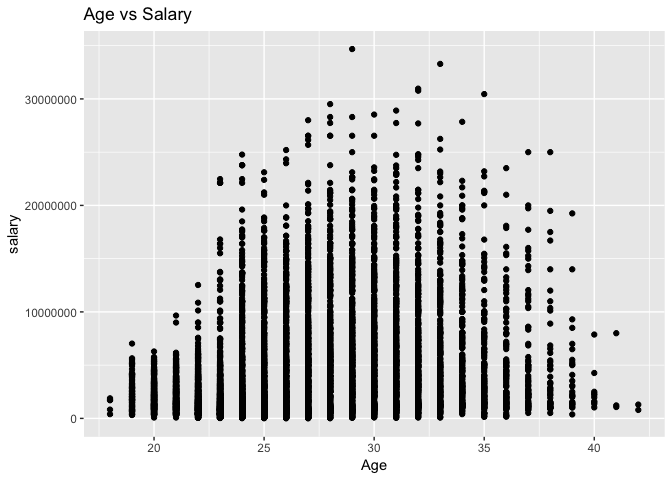
\includegraphics{nba_data_visV4_files/figure-latex/unnamed-chunk-13-1.pdf}

Lets look at over 51 percent EFG

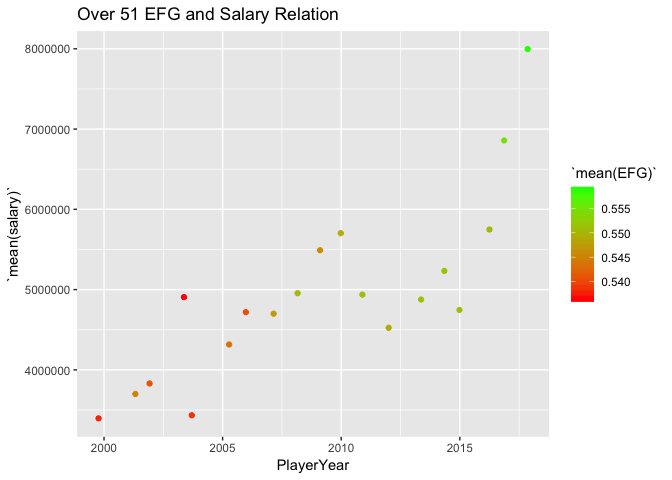
\includegraphics{nba_data_visV4_files/figure-latex/unnamed-chunk-14-1.pdf}

Early on EFG didn't seem to take notice to teams as much, but as we
entered the 2014 year and above this statisic became more relevant

\subsubsection{Which schools in the US are teams spending their salary
the most for
salary.}\label{which-schools-in-the-us-are-teams-spending-their-salary-the-most-for-salary.}

Exploring this data could give us information on where to look to draft
a NBA prospect for a NBA team.

\begin{verbatim}
##  [1] "Alabama"                  "Alabama A&M"             
##  [3] "Alabama-Birmingham"       "Alabama-Huntsville"      
##  [5] "American International"   "Arizona"                 
##  [7] "Arizona State"            "Arkansas"                
##  [9] "Arkansas-Little Rock"     "Auburn"                  
## [11] "Auburn-Montgomery"        "Augsburg"                
## [13] "Austin Peay"              "Ball State"              
## [15] "Barton Community College" "Baylor"                  
## [17] "Belmont"                  "Blinn"                   
## [19] "Boise State"              "Boston College"
\end{verbatim}

249 schools (no school included for internationals if they played
professionally outside the USA)

Lets look at the top 10 schools that got paid

\begin{verbatim}
## # A tibble: 11 x 3
##    school         count_school     salary
##    <fct>                 <int>      <dbl>
##  1 None                   1285 7407695183
##  2 Kentucky                261 1220596079
##  3 Duke                    252 1308479631
##  4 North Carolina          241 1182185814
##  5 UCLA                    206  947159451
##  6 Kansas                  194  840093830
##  7 Arizona                 190  995023686
##  8 Connecticut             184 1038212650
##  9 Florida                 143  817700613
## 10 Georgia Tech            129  718884989
## 11 Texas                   116  627431018
\end{verbatim}

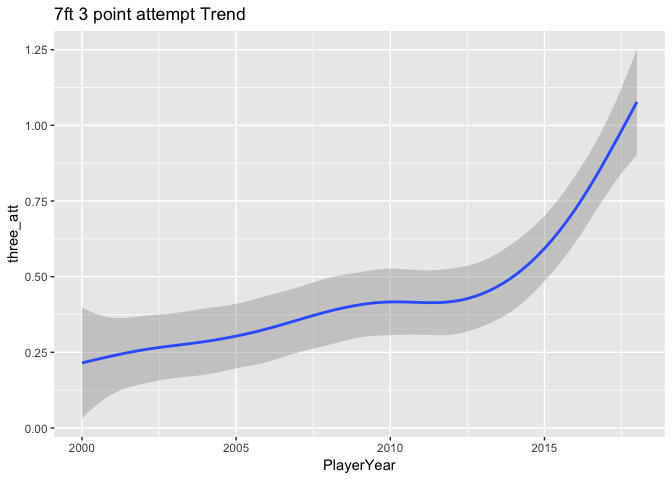
\includegraphics{nba_data_visV4_files/figure-latex/unnamed-chunk-16-1.pdf}

Should be always looking at these schools for prospects looking at the
total salary paid. Seems to have best basketball programs

Lets take a look at the data that was accounted for by college programs

Looking at the notable names Lebron James, Kobe Bryant, Kevin Garnett,
Dwight Howard, Jermaine O'neal that would be 5 out of 430 highschoolers
who made it to superstar level. That's 1.2 percent chance.

Out of Country Prospects for teams to spend their salary on.

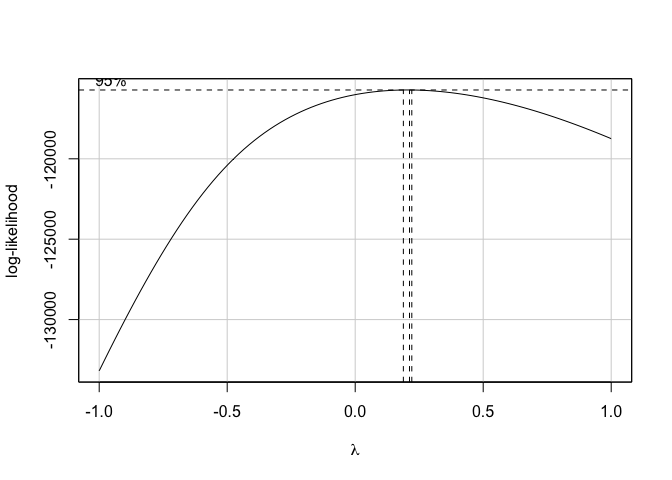
\includegraphics{nba_data_visV4_files/figure-latex/unnamed-chunk-18-1.pdf}

Looking at the top salaries would want to look into these countries in
terms if finding talent or drafting in the future or free agents.

\subsubsection{How important is getting the number 1 pick by either
saving salary by tanking or being
unlucky}\label{how-important-is-getting-the-number-1-pick-by-either-saving-salary-by-tanking-or-being-unlucky}

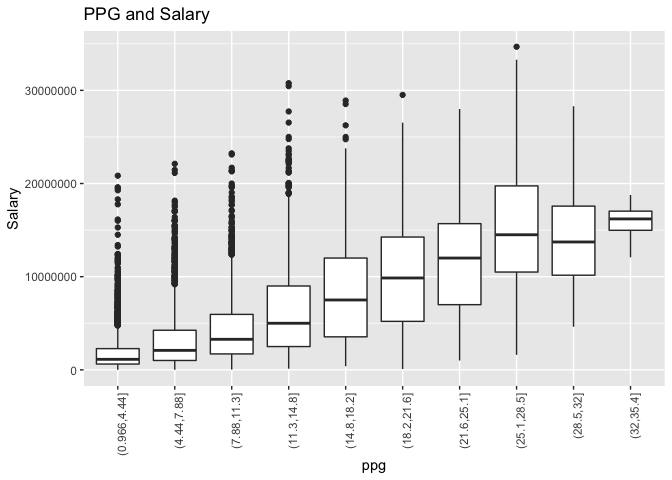
\includegraphics{nba_data_visV4_files/figure-latex/unnamed-chunk-19-1.pdf}

Now lets compare to being a relatively good team but paying for good
scouts to draft or look abroad in the second round.

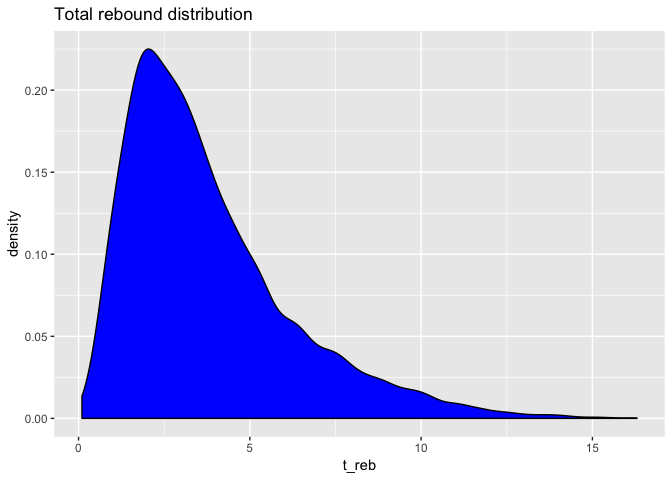
\includegraphics{nba_data_visV4_files/figure-latex/unnamed-chunk-20-1.pdf}

We can see that by not selecting the number one pick overall it yielded
4 more defensive players or nba team selections. But we have to keep in
mind other picks in the first round. Other notable picks that aren't
first rounders include Stephen Curry, Kevin Durant, A'mare Stoudamire.

\subsubsection{The Best vs the Worst}\label{the-best-vs-the-worst}

Lets look at the data for the winning team and team that lost the most
for each year 2000 to 2018
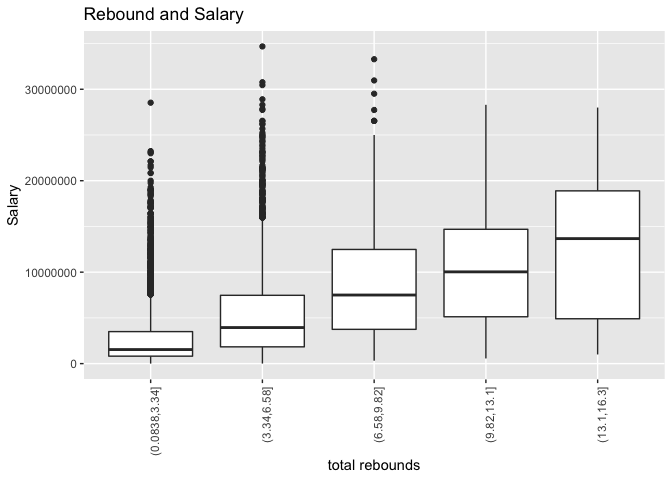
\includegraphics{nba_data_visV4_files/figure-latex/unnamed-chunk-21-1.pdf}
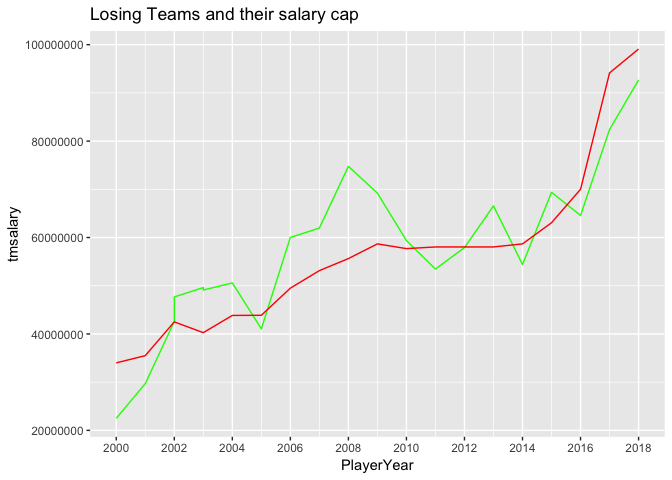
\includegraphics{nba_data_visV4_files/figure-latex/unnamed-chunk-21-2.pdf}

Winning teams tend to spend over the cap while losing teams spend under
or stay below the salary cap for each year.

Lets look at the Top teams each year vs Worst teams each year

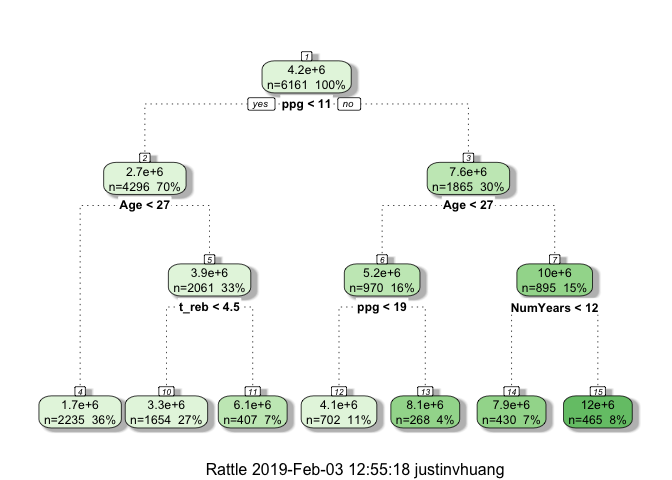
\includegraphics{nba_data_visV4_files/figure-latex/unnamed-chunk-22-1.pdf}
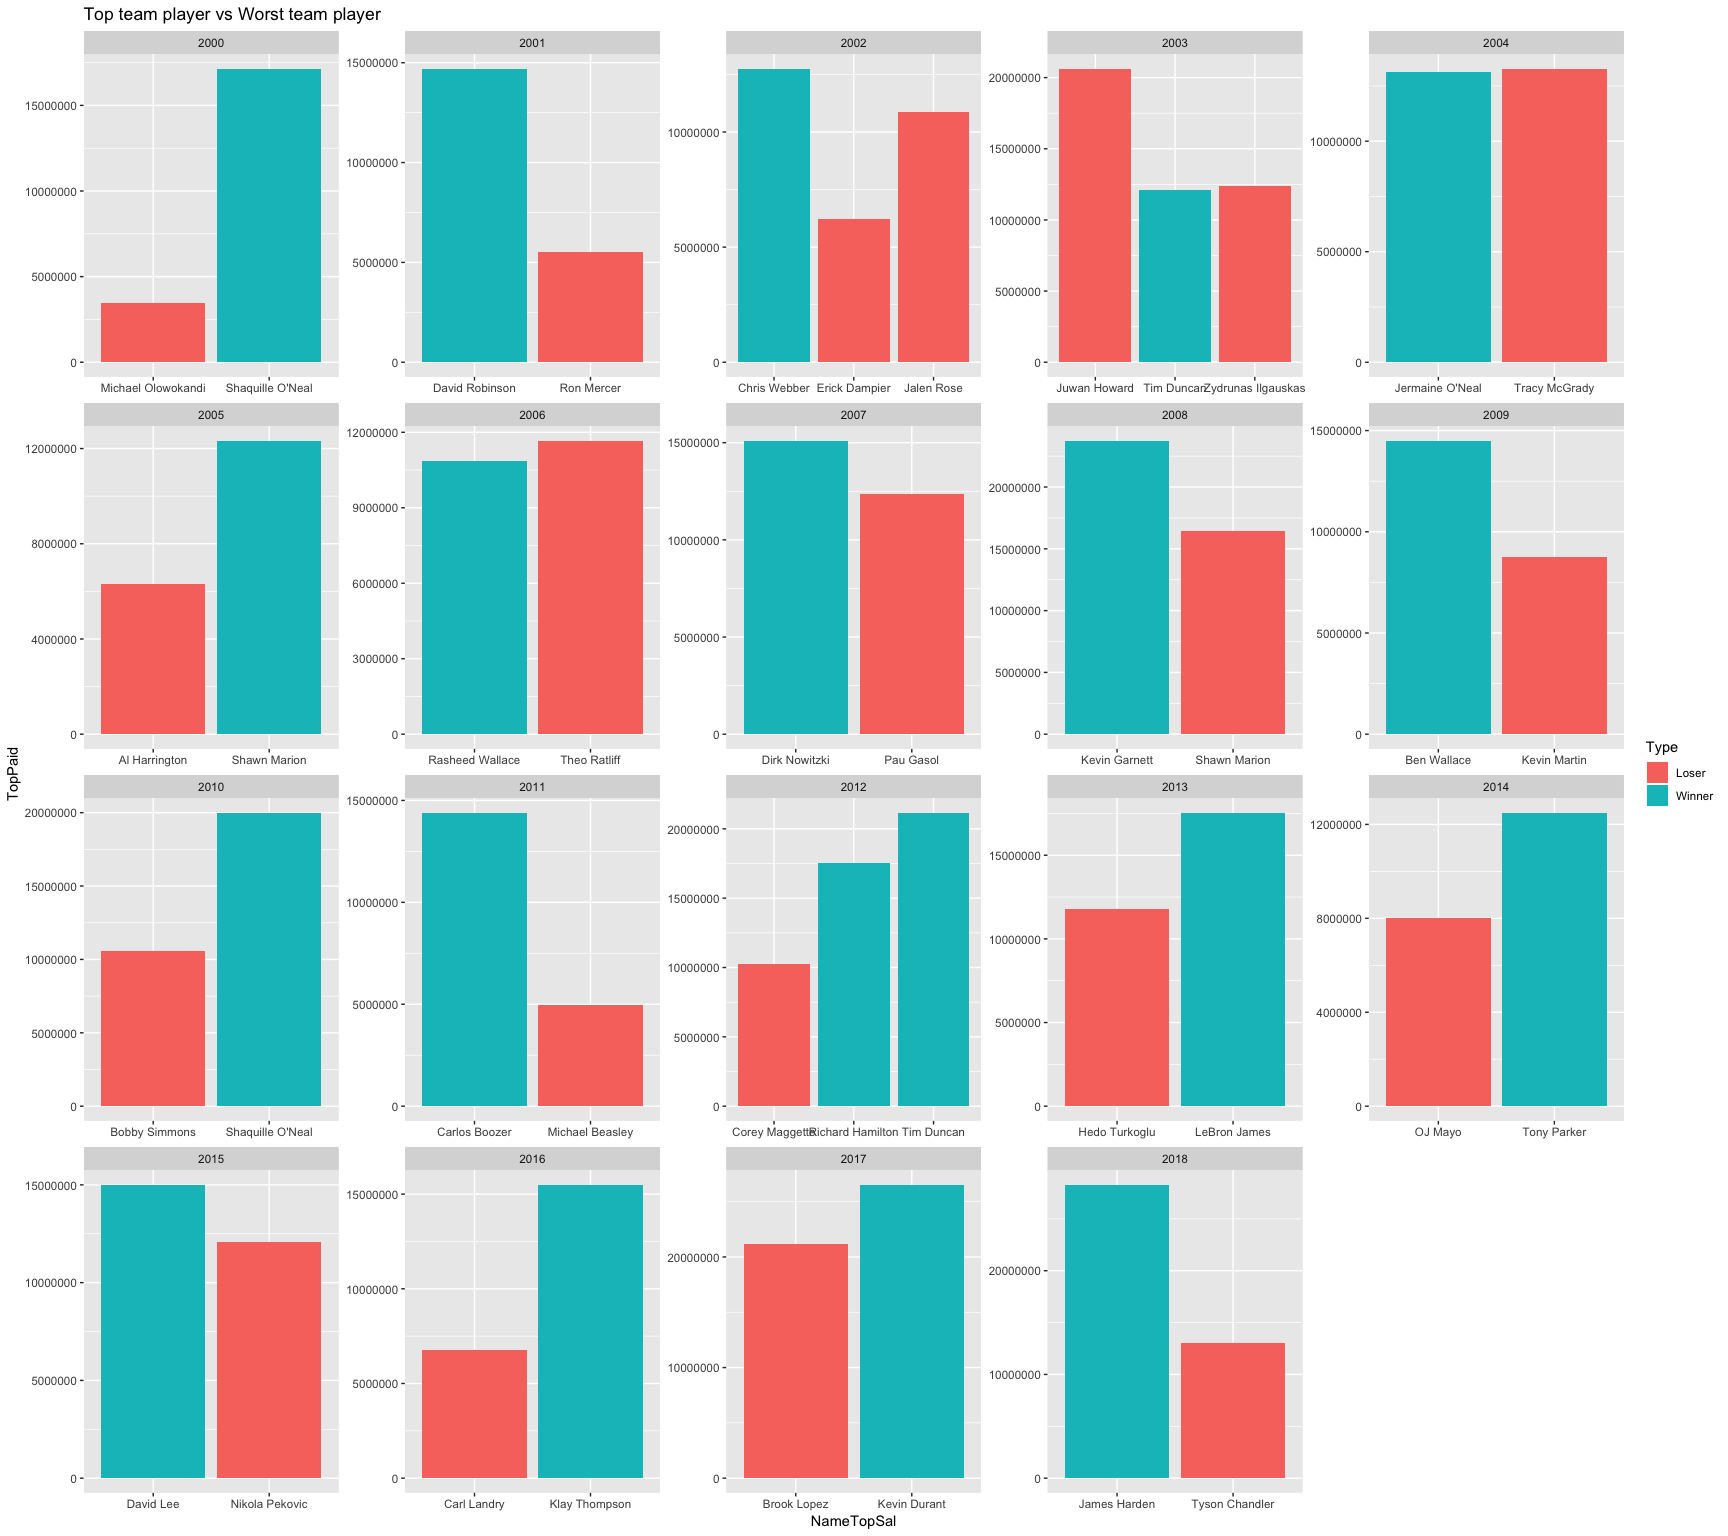
\includegraphics{nba_data_visV4_files/figure-latex/unnamed-chunk-22-2.pdf}
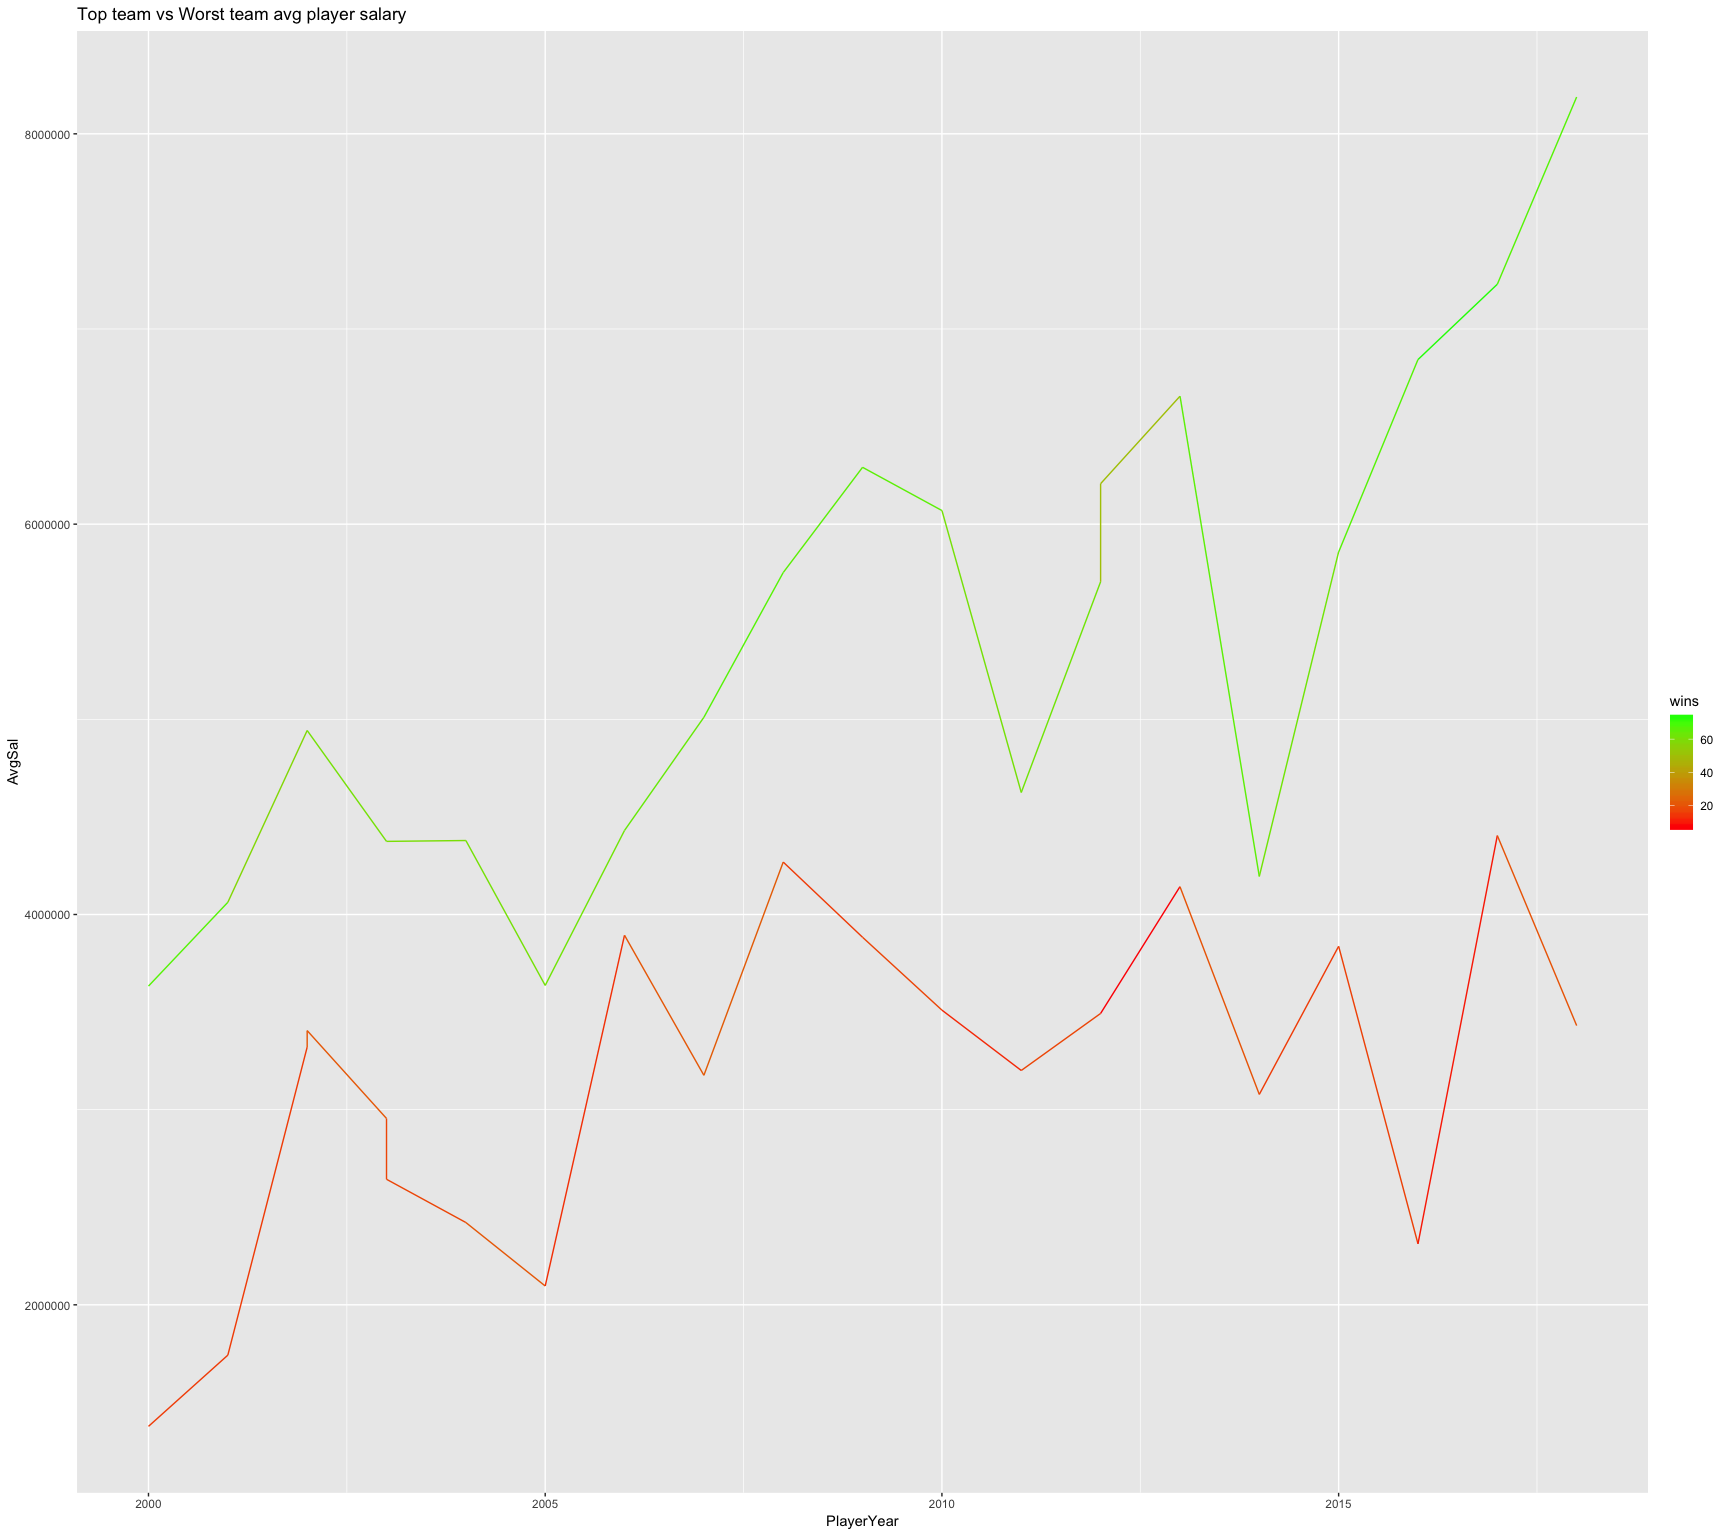
\includegraphics{nba_data_visV4_files/figure-latex/unnamed-chunk-22-3.pdf}

We can see the top teams spend the most money each year. Their best
players also recieve the more money than the worst teams player. Looking
at the average salary the best teams spend much more than the worst.

\subsubsection{Most successful teams in the last 19
years.}\label{most-successful-teams-in-the-last-19-years.}

Looking at the team that spent the most over and the team that spent the
least.

Looking at the winningest team vs the team that lost the most in the
last 19 years.

The team that won the most is the 2016 GSW and the team with the fewest
wins was the 2012 Charlotte Bobcats. The team that spent the most over
the salary cap was the 2018 Cleveland Caviliers. The team that spent the
least over the salary cap was the 2000 LA clippers.

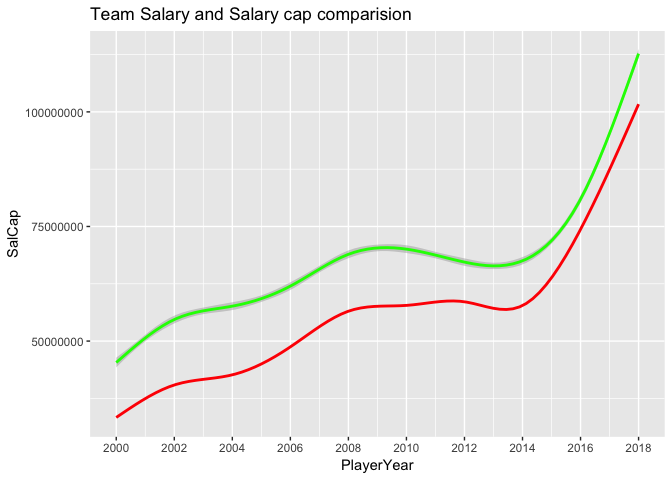
\includegraphics{nba_data_visV4_files/figure-latex/unnamed-chunk-23-1.pdf}

\begin{verbatim}
## # A tibble: 14 x 6
## # Groups:   salary [14]
##    name                   salary   ppg   EFG t_reb PlusMinus
##    <fct>                   <int> <dbl> <dbl> <dbl>     <dbl>
##  1 Klay Thompson        15501000  22.1 0.569   3.8      14.7
##  2 Draymond Green       14260870  14   0.554   9.5      18  
##  3 Andrew Bogut         12000000   5.4 0.625   7        13.9
##  4 Andre Iguodala       11710456   7   0.544   4        13.2
##  5 Stephen Curry        11370786  30.1 0.631   5.4      17.7
##  6 Anderson Varejao     10158574   2.6 0.435   2.7       2.6
##  7 Shaun Livingston      5543725   6.3 0.531   2.2       7  
##  8 Harrison Barnes       3873398  11.7 0.531   4.9      10.5
##  9 Marreese Speights     3815500   7.1 0.452   3.3       1.2
## 10 Leandro Barbosa       2500000   6.4 0.519   1.7       2.4
## 11 Festus Ezeli          2008748   7   0.54    5.6      14.6
## 12 Brandon Rush          1270964   4.2 0.542   2.5      -0.9
## 13 Ian Clark              947276   3.6 0.5     1        -7.3
## 14 James Michael McAdoo   845059   2.9 0.55    1.4     -15.9
\end{verbatim}

\begin{verbatim}
##      total  TopPaid    NameTopSal highscore    NameTopPpg efficient
## 1 95806356 15501000 Klay Thompson      30.1 Stephen Curry 0.6311881
##      NameTopEFG HighPlusMinus      NameTopPM LeastPaid
## 1 Stephen Curry            18 Draymond Green    845059
##             NameLowSal  AvgSal tmsalary   salcap OverUnder wins
## 1 James Michael McAdoo 6843311 93669566 70000000  1.338137   73
\end{verbatim}

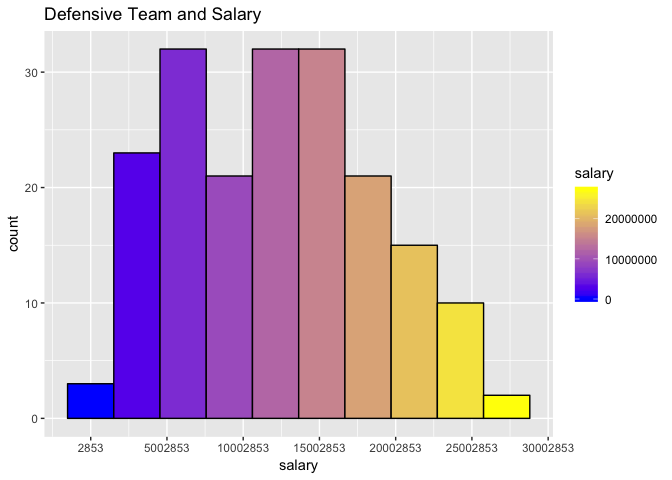
\includegraphics{nba_data_visV4_files/figure-latex/unnamed-chunk-23-2.pdf}

From the greenline we can see that team salary has stayed above salary
cap.

Lets see how they drafted in the last 19 years

\begin{verbatim}
##                  name  salary  ppg       EFG
## 104    Antawn Jamison 2503800 19.6 0.4715909
## 1564 Jason Richardson 2607360 15.6 0.4612676
## 1746        JR Bremer  563679  3.3 0.3295455
## 4732    Stephen Curry 2913840 18.6 0.5492958
## 5358    Klay Thompson 2222160 16.6 0.5102041
## 5813  Harrison Barnes 2923920  9.5 0.4482759
\end{verbatim}

They also successfully drafted Draymond Green who won defensive player
of the year.

Looking at the worst team in NBA history

\begin{verbatim}
## # A tibble: 14 x 6
## # Groups:   salary [14]
##    name               salary   ppg   EFG t_reb PlusMinus
##    <fct>               <int> <dbl> <dbl> <dbl>     <dbl>
##  1 Corey Maggette   10262069  15   0.402   3.9     -15.4
##  2 Tyrus Thomas      7305765   5.6 0.361   3.7     -14.4
##  3 DeSagana Diop     6925400   1.1 0.375   3.1     -19.1
##  4 Matt Carroll      3900000   2.7 0.367   1.1     -11.9
##  5 DJ Augustin       3236470  11.1 0.441   2.3     -14.7
##  6 Bismack Biyombo   2798040   5.2 0.455   5.8     -16  
##  7 Eduardo Najera    2750000   2.6 0.448   2.3      -7.2
##  8 Reggie Williams   2500000   8.3 0.481   2.8     -18.4
##  9 Kemba Walker      2356320  12.1 0.414   3.5     -14.3
## 10 Gerald Henderson  2250600  15.1 0.466   4.1     -13.7
## 11 DJ White          2001167   6.8 0.492   3.6     -15.3
## 12 Byron Mullens     1288200   9.3 0.440   5       -12.4
## 13 Derrick Brown      854389   8.1 0.532   3.6     -13  
## 14 Cory Higgins       473604   3.9 0.345   0.9     -12.9
\end{verbatim}

\begin{verbatim}
##      total  TopPaid     NameTopSal highscore       NameTopPpg efficient
## 1 48902024 10262069 Corey Maggette      15.1 Gerald Henderson  0.531746
##      NameTopEFG HighPlusMinus      NameTopPM LeastPaid   NameLowSal
## 1 Derrick Brown          -7.2 Eduardo Najera    473604 Cory Higgins
##    AvgSal tmsalary   salcap OverUnder wins
## 1 3493002 57902024 58044000  0.997554    7
\end{verbatim}

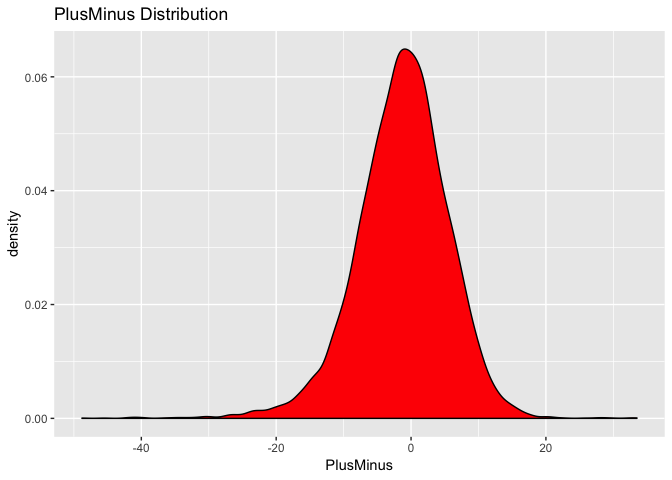
\includegraphics{nba_data_visV4_files/figure-latex/unnamed-chunk-25-1.pdf}

You can see Michael Jordan didn't really spend that much money on his
bobcats to have them winning.

Comparing the worst vs the best team side by side

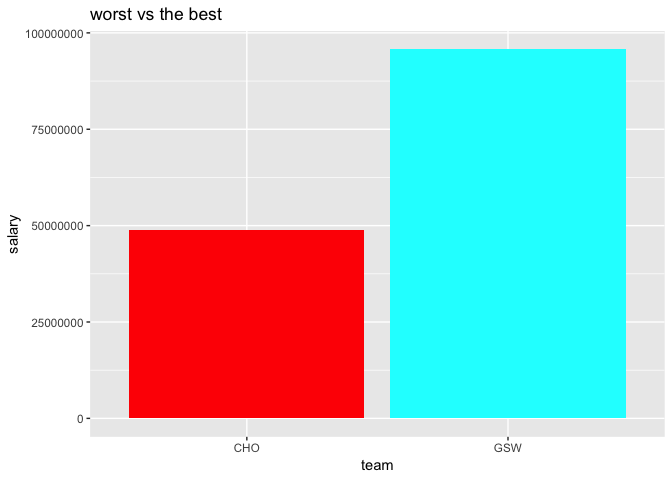
\includegraphics{nba_data_visV4_files/figure-latex/unnamed-chunk-26-1.pdf}

The GSW looked as if they spent double the amount. But also have to
include the salary cap increase. Teams with winning players will spend
more over the cap than teams who can't win. The real question is do
teams spend just enough to stay in cap and then just tank to get draft
picks and then players?

Looking at the max salary offender

\begin{verbatim}
##      team PlayerYear
## 7508  CLE       2018
## 7509  CLE       2018
## 7510  CLE       2018
## 7514  CLE       2018
## 7520  CLE       2018
## 7538  CLE       2018
## 7539  CLE       2018
## 7552  CLE       2018
## 7772  CLE       2018
## 7773  CLE       2018
## 7774  CLE       2018
## 7775  CLE       2018
## 7776  CLE       2018
## 7777  CLE       2018
## 7778  CLE       2018
\end{verbatim}

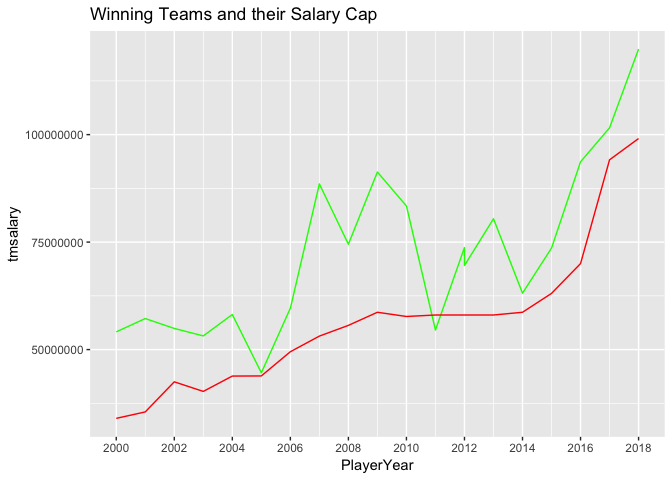
\includegraphics{nba_data_visV4_files/figure-latex/unnamed-chunk-27-1.pdf}

\begin{verbatim}
##       total  TopPaid   NameTopSal highscore   NameTopPpg efficient
## 1 138780646 33285709 LeBron James      27.5 LeBron James 0.7142857
##   NameTopEFG HighPlusMinus   NameTopPM LeastPaid   NameLowSal  AvgSal
## 1 Ante Zizic           7.9 Kyle Korver     77250 John Holland 9252043
##    tmsalary   salcap OverUnder wins
## 1 137722926 99093000  1.389835   50
\end{verbatim}

\begin{verbatim}
##     team PlayerYear
## 179  LAC       2000
## 180  LAC       2000
## 181  LAC       2000
## 182  LAC       2000
## 183  LAC       2000
## 184  LAC       2000
## 185  LAC       2000
## 186  LAC       2000
## 187  LAC       2000
## 217  LAC       2000
## 256  LAC       2000
## 258  LAC       2000
## 259  LAC       2000
## 281  LAC       2000
## 282  LAC       2000
\end{verbatim}

\begin{verbatim}
## # A tibble: 15 x 6
## # Groups:   salary [12]
##    name                salary   ppg   EFG t_reb PlusMinus
##    <fct>                <int> <dbl> <dbl> <dbl>     <dbl>
##  1 Michael Olowokandi 3456240   9.8 0.432   8.2     -13.8
##  2 Tyrone Nesby       2716667  13.3 0.452   3.8     -13.2
##  3 Lamar Odom         2445480  16.6 0.467   7.8      -7.5
##  4 Eric Piatkowski    2000000   8.7 0.5     3       -12.6
##  5 Eric Murdock       1925000   5.6 0.431   1.9     -10.3
##  6 Keith Closs        1680000   4.2 0.486   3.1     -10.6
##  7 Derek Anderson     1439400  16.9 0.474   4       -13.1
##  8 Maurice Taylor     1367400  17.1 0.465   6.5     -12.8
##  9 Brian Skinner       843000   5.4 0.512   6.1      -6.6
## 10 Anthony Avent       510000   1.7 0.3     1.5      -8.3
## 11 Pete Chilcutt       510000   2.1 0.413   2.3     -12.1
## 12 Troy Hudson         460000   8.8 0.437   2.4     -10.9
## 13 Etdrick Bohannon    460000   2.2 0.5     2.4     -13.6
## 14 Jeff McInnis        460000   7.2 0.453   2.9     -13.3
## 15 Charles R Jones     385000   3.4 0.431   1.1     -12.1
\end{verbatim}

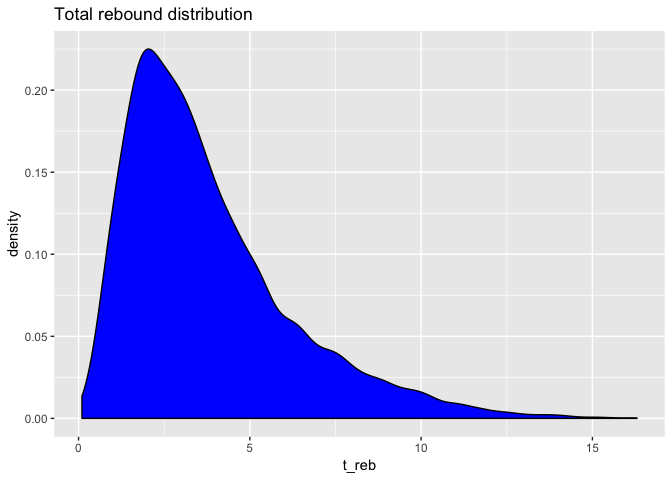
\includegraphics{nba_data_visV4_files/figure-latex/unnamed-chunk-28-1.pdf}

\begin{verbatim}
##      total TopPaid         NameTopSal highscore     NameTopPpg efficient
## 1 20658187 3456240 Michael Olowokandi      17.1 Maurice Taylor 0.5121951
##      NameTopEFG HighPlusMinus     NameTopPM LeastPaid      NameLowSal
## 1 Brian Skinner          -6.6 Brian Skinner    385000 Charles R Jones
##    AvgSal tmsalary   salcap OverUnder wins
## 1 1377212 22489343 34000000 0.6614513   15
\end{verbatim}

\begin{verbatim}
##                    name  salary  ppg       EFG
## 186  Michael Olowokandi 3456240  9.8 0.4315789
## 775          Lamar Odom 2628960 17.2 0.4963768
## 1059       Darius Miles 3054840  9.5 0.4871795
## 3942        Eric Gordon 2623200 16.1 0.5301724
## 3943        Al Thornton 1776240 16.8 0.4560811
## 4095        Eric Gordon 2819880 16.9 0.5277778
## 5085       Eric Bledsoe 1596360  3.3 0.4062500
## 5123      Blake Griffin 5731080 20.7 0.5483871
\end{verbatim}

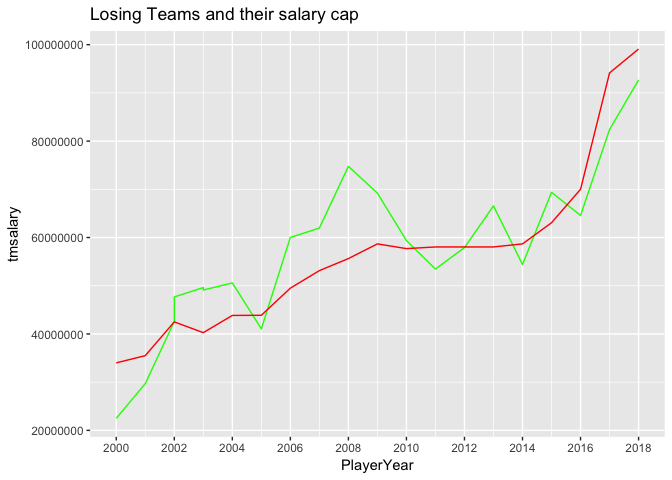
\includegraphics{nba_data_visV4_files/figure-latex/unnamed-chunk-28-2.pdf}

The Clippers drafted well with Blake Griffin however there were many
injuries. So tanking to get a star was worth it. They also got Eric
Gordon and Lamar Odom who both woth 6th man of the year.

Comparing them with the Cavs. We can see the Cavs spent money to keep
their team intact for their Finals run.

\subsubsection{Comparing the Average
Joe}\label{comparing-the-average-joe}

\begin{verbatim}
##      height   weight  salary  plusMinus      age    games    start
## 1  200.9356 222.0764 2880067 -1.1627685 27.74702 58.84248 28.57518
## 2  200.9545 222.6364 3398885 -1.2510101 27.72727 59.10859 29.96465
## 3  201.5609 224.6878 3487920 -0.9461929 27.18782 58.99239 29.94162
## 4  201.6292 224.7008 3783693 -0.9245524 27.12788 60.20716 30.38875
## 5  201.3472 224.0000 3817195 -0.9489637 27.13731 59.93782 30.67098
## 6  201.4734 224.2488 3911320 -1.5695652 26.94928 58.76570 29.57729
## 7  201.0049 223.2469 4091303 -1.2205379 26.54279 59.48166 30.03912
## 8  200.6675 222.7530 4140794 -1.2315914 26.44893 58.72922 29.19002
## 9  200.8610 222.3325 4574357 -1.1846154 26.84367 59.01985 29.46402
## 10 201.2897 223.0907 4715669 -1.4602015 26.57683 59.11839 30.14106
## 11 200.9824 222.8643 4829387 -1.1979899 26.63065 59.36181 29.98744
## 12 201.3957 224.0192 4560710 -1.2580336 26.63309 59.46043 29.47242
## 13 200.9750 222.8636 4348460 -1.7250000 26.58182 46.56591 22.44545
## 14 200.8822 222.1455 4447435 -1.1697460 26.74134 58.67206 28.35566
## 15 200.9120 221.4718 4402763 -1.0440181 26.56208 56.99097 27.74266
## 16 200.8978 221.3244 4430783 -1.5308889 26.68667 56.22222 26.72444
## 17 201.1982 221.5248 5097982 -1.4074324 26.71171 57.95045 27.69369
## 18 201.1186 220.4295 6218880 -1.3767338 26.44743 57.69128 27.50336
## 19 200.5735 218.2668 6450838 -1.6067227 26.18697 54.02731 25.83193
##        mins       fg   fg_att    fg_per     three three_att three_per
## 1  21.36683 3.163962 7.130549 0.4365386 0.4152745  1.196897 0.3469591
## 2  22.04369 3.172980 7.226768 0.4314876 0.4270202  1.214646 0.3515593
## 3  22.13680 3.268528 7.395939 0.4361455 0.4573604  1.315990 0.3475410
## 4  21.92558 3.178517 7.233504 0.4312024 0.4498721  1.297954 0.3466010
## 5  22.43523 3.219689 7.393523 0.4314557 0.4694301  1.368135 0.3431168
## 6  22.23430 3.242995 7.316908 0.4368336 0.4985507  1.423430 0.3502461
## 7  22.09927 3.220049 7.142787 0.4449107 0.5051345  1.422005 0.3552270
## 8  21.78147 3.243468 7.123278 0.4489531 0.5399050  1.519952 0.3552118
## 9  21.88462 3.283623 7.260794 0.4452385 0.5727047  1.604963 0.3568336
## 10 22.30428 3.368766 7.394207 0.4500620 0.5881612  1.620907 0.3628594
## 11 22.20503 3.392211 7.397990 0.4549261 0.5753769  1.642714 0.3502600
## 12 21.86355 3.294005 7.226859 0.4536585 0.5693046  1.598801 0.3560822
## 13 21.37068 3.148636 7.088636 0.4374295 0.5572727  1.616364 0.3447694
## 14 21.42471 3.220785 7.195150 0.4430161 0.6217090  1.771824 0.3508863
## 15 21.31603 3.255305 7.228217 0.4441381 0.6706546  1.890745 0.3547039
## 16 21.10867 3.213556 7.233111 0.4399928 0.6842222  1.974444 0.3465391
## 17 21.10946 3.279054 7.300450 0.4472961 0.7204955  2.056081 0.3504217
## 18 20.98277 3.321477 7.314989 0.4507245 0.8192394  2.313423 0.3541244
## 19 20.86660 3.341807 7.363445 0.4518979 0.8915966  2.509244 0.3553248
##         two  two_att   two_per       efg       ft   ft_att    ft_per
## 1  2.751551 5.931981 0.4533731 0.4636205 1.614797 2.168258 0.7447441
## 2  2.744192 6.006566 0.4447630 0.4589386 1.648737 2.220202 0.7426069
## 3  2.808376 6.078426 0.4528598 0.4633263 1.612183 2.154569 0.7482625
## 4  2.725064 5.936829 0.4467322 0.4589927 1.635806 2.171355 0.7533569
## 5  2.749223 6.030570 0.4465291 0.4599201 1.655181 2.217098 0.7465529
## 6  2.745652 5.896135 0.4558527 0.4670815 1.766184 2.355556 0.7497949
## 7  2.713692 5.719560 0.4639777 0.4762883 1.755990 2.367726 0.7416357
## 8  2.705226 5.605463 0.4710350 0.4836586 1.746793 2.325653 0.7510979
## 9  2.708189 5.654839 0.4662997 0.4822767 1.661042 2.228040 0.7455173
## 10 2.779597 5.770277 0.4695675 0.4879611 1.702519 2.234509 0.7619209
## 11 2.816834 5.754020 0.4830450 0.4916816 1.676131 2.223367 0.7538705
## 12 2.724460 5.628537 0.4743616 0.4914891 1.623501 2.148681 0.7555804
## 13 2.590455 5.472045 0.4634083 0.4749558 1.461364 1.953636 0.7480223
## 14 2.603233 5.422171 0.4720255 0.4849253 1.447575 1.937644 0.7470799
## 15 2.584424 5.334989 0.4844292 0.4899395 1.517156 2.014221 0.7532220
## 16 2.530889 5.258444 0.4724925 0.4866008 1.461333 1.960222 0.7454937
## 17 2.559910 5.245045 0.4820120 0.4949224 1.518919 2.022973 0.7508350
## 18 2.503803 5.000447 0.4925256 0.5044656 1.513199 1.970470 0.7679382
## 19 2.448950 4.857143 0.4964841 0.5103584 1.409874 1.842437 0.7652223
##        o_reb    d_reb    t_reb   assist     steal     block       TO
## 1  1.1193317 2.684964 3.805489 1.926969 0.6947494 0.4441527 1.308115
## 2  1.1022727 2.782576 3.886616 1.927273 0.7131313 0.4750000 1.305303
## 3  1.1390863 2.761929 3.899239 1.955838 0.7104061 0.4794416 1.269543
## 4  1.1153453 2.731202 3.843223 1.909719 0.7150895 0.4659847 1.291816
## 5  1.1341969 2.789637 3.920466 1.946891 0.7300518 0.4608808 1.335233
## 6  1.1128019 2.739372 3.853382 1.914010 0.6917874 0.4492754 1.279710
## 7  1.0273839 2.715648 3.739120 1.831051 0.6562347 0.4283619 1.264792
## 8  1.0049881 2.682423 3.686698 1.876960 0.6539192 0.4121140 1.311639
## 9  1.0317618 2.776427 3.806700 1.949132 0.6625310 0.4344913 1.232506
## 10 1.0423174 2.806297 3.847355 1.875819 0.6690176 0.4632242 1.237028
## 11 1.0288945 2.821608 3.848995 1.907035 0.6600503 0.4555276 1.243970
## 12 1.0074341 2.775300 3.779376 1.876499 0.6565947 0.4510791 1.229976
## 13 1.0027273 2.702045 3.701364 1.835682 0.6779545 0.4477273 1.238182
## 14 0.9921478 2.727945 3.721247 1.934180 0.6866051 0.4533487 1.228176
## 15 0.9629797 2.783070 3.747178 1.915124 0.6717833 0.4164786 1.249661
## 16 0.9446667 2.802889 3.741111 1.905333 0.6786667 0.4097778 1.198889
## 17 0.9121622 2.896622 3.803153 1.929505 0.6826577 0.4344595 1.209459
## 18 0.8870246 2.876957 3.762640 1.930425 0.6657718 0.4105145 1.157271
## 19 0.8352941 2.870798 3.704202 1.993277 0.6739496 0.4115546 1.181513
##       fouls      ppg PlayerYear
## 1  2.126730 8.356086       2000
## 2  2.092424 8.421970       2001
## 3  1.990609 8.605330       2002
## 4  2.036829 8.443223       2003
## 5  2.034197 8.566062       2004
## 6  2.151691 8.751691       2005
## 7  2.141565 8.699022       2006
## 8  2.047743 8.775534       2007
## 9  1.960794 8.801737       2008
## 10 1.987406 9.029723       2009
## 11 1.983668 9.028141       2010
## 12 1.943405 8.773621       2011
## 13 1.779545 8.311364       2012
## 14 1.800231 8.513395       2013
## 15 1.869074 8.694808       2014
## 16 1.807778 8.568444       2015
## 17 1.811486 8.797523       2016
## 18 1.768680 8.970694       2017
## 19 1.753782 8.973319       2018
\end{verbatim}

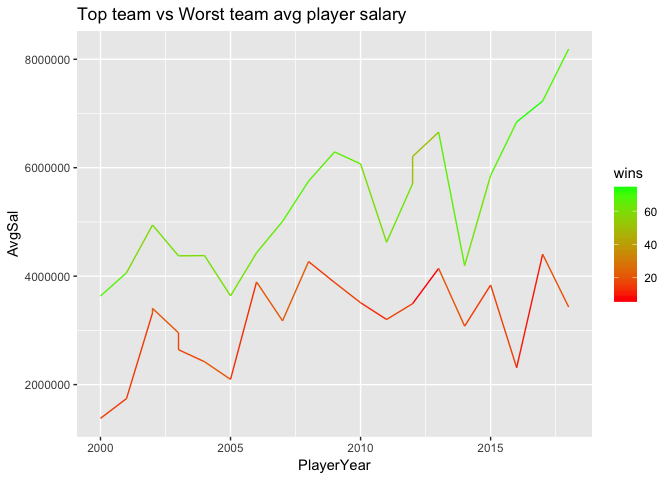
\includegraphics{nba_data_visV4_files/figure-latex/unnamed-chunk-29-1.pdf}

\begin{verbatim}
##     name   height   weight  salary plusMinus      age    games   start
## 1 AvgJoe 201.0873 222.5623 4399392 -1.274556 26.81424 57.84977 28.6163
##      mins      fg   fg_att    fg_per     three three_att three_per
## 1 21.7084 3.25418 7.261427 0.4429425 0.5806992  1.650448 0.3515404
##        two two_att   two_per       efg       ft   ft_att    ft_per
## 1 2.673354 5.61071 0.4679881 0.4806002 1.601489 2.132454 0.7511976
##      o_reb    d_reb    t_reb   assist    steal     block       TO    fouls
## 1 1.021201 2.775143 3.794608 1.912669 0.681629 0.4422839 1.251199 1.951981
##       ppg
## 1 8.68851
\end{verbatim}

Above is the chart of taking all the players and averaging them all out
to create Mr.~Avg Joe. Now lets compare him to differnt categories of
NBA players.

\subsubsection{Average Joe vs Superstar, Star and
Roleplayer}\label{average-joe-vs-superstar-star-and-roleplayer}

SuperStars

Looking at the life cycle of a NBA player we can determine a salary
reference point of how to pay them.

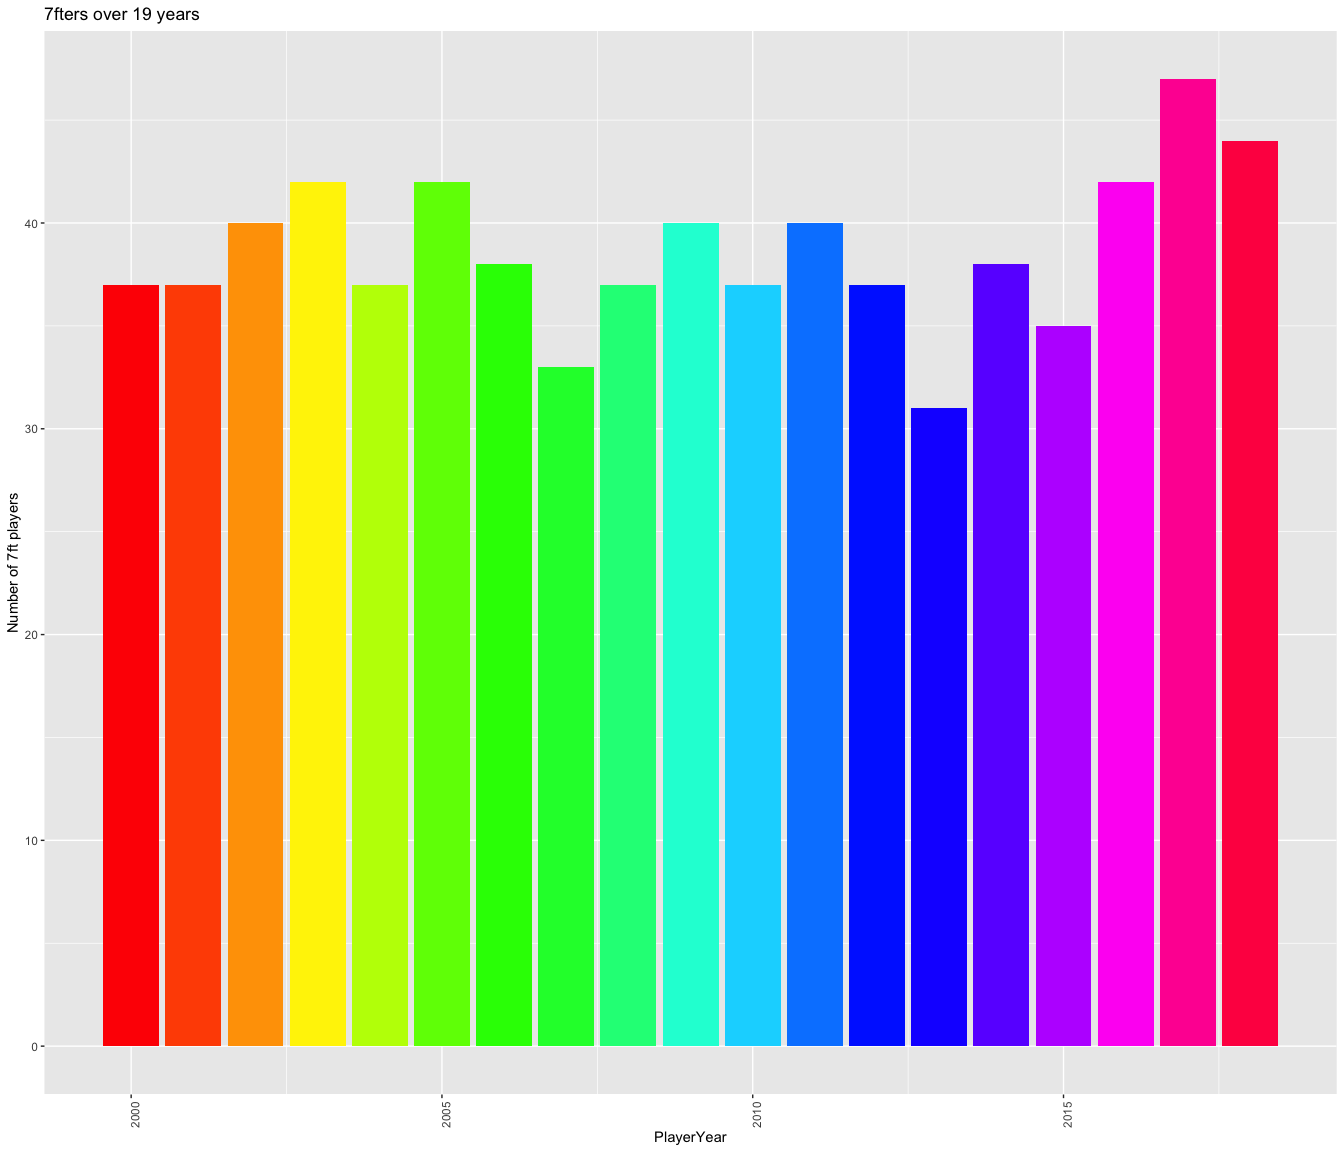
\includegraphics{nba_data_visV4_files/figure-latex/unnamed-chunk-30-1.pdf}

Duncan salary and production is above the average player. Late in his
career he took pay cuts which brought his salary down.

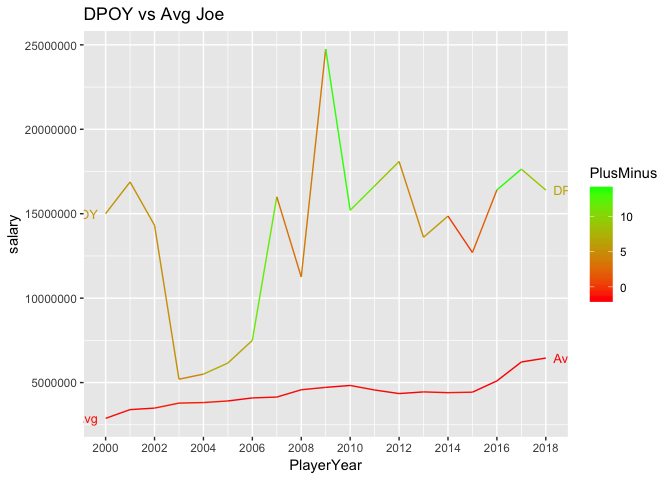
\includegraphics{nba_data_visV4_files/figure-latex/unnamed-chunk-31-1.pdf}

Kobe commanded a much higher salary than the avg Joe. He also did not
take a decrease in salary for the later years. However his minutes per
game did not go down. It might be interesting to do an analysis on his
achillies injury and overuse of his body in future analysis.

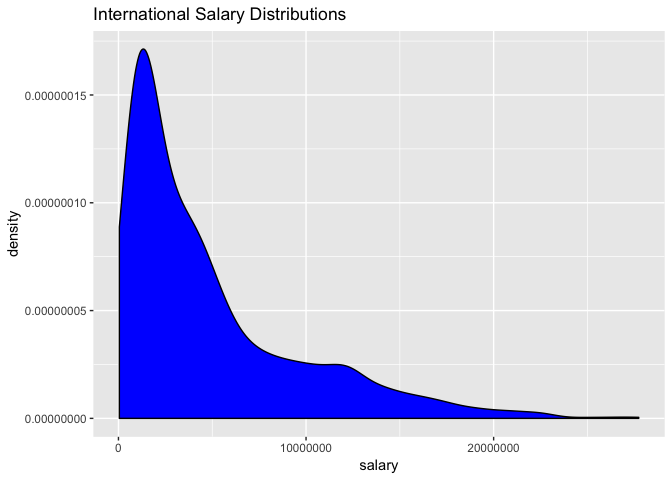
\includegraphics{nba_data_visV4_files/figure-latex/unnamed-chunk-32-1.pdf}

Lebron salary has kept going up. His body has not slowed down either.
The amount of minutes played has not really decreased at all. Seems like
a player anomally.

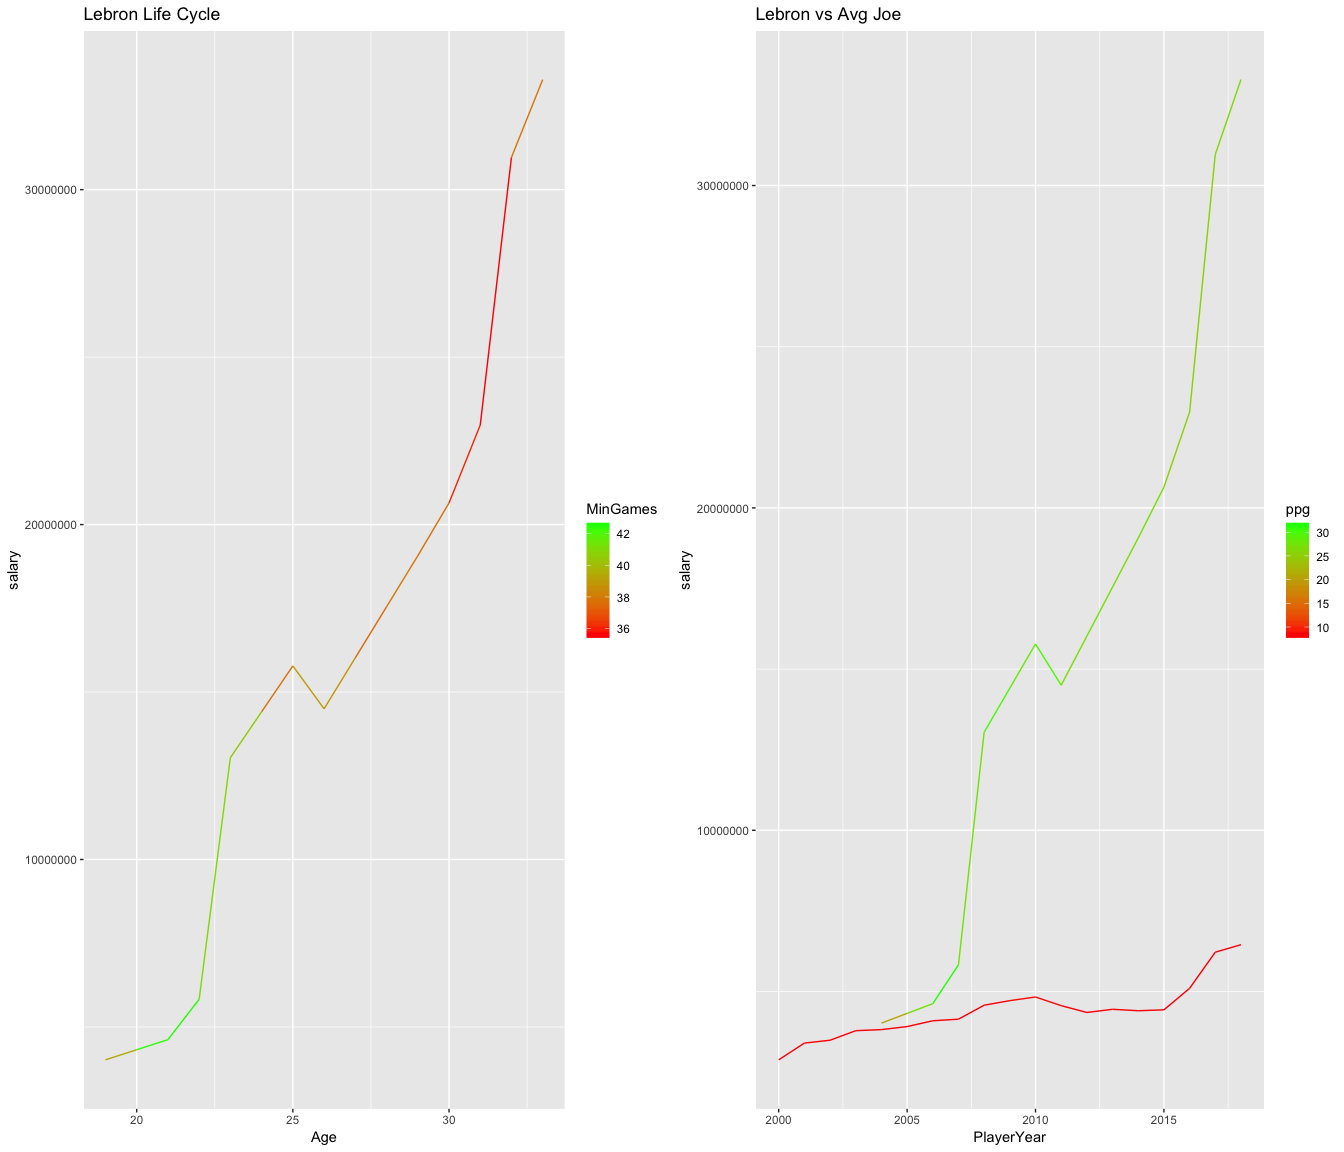
\includegraphics{nba_data_visV4_files/figure-latex/unnamed-chunk-33-1.pdf}

Garnett seems to have taken a few paycuts for the Timberwolves to get
him better players. Production did go down a lot. Perhaps bigmen have
smaller life cycles than smaller players.

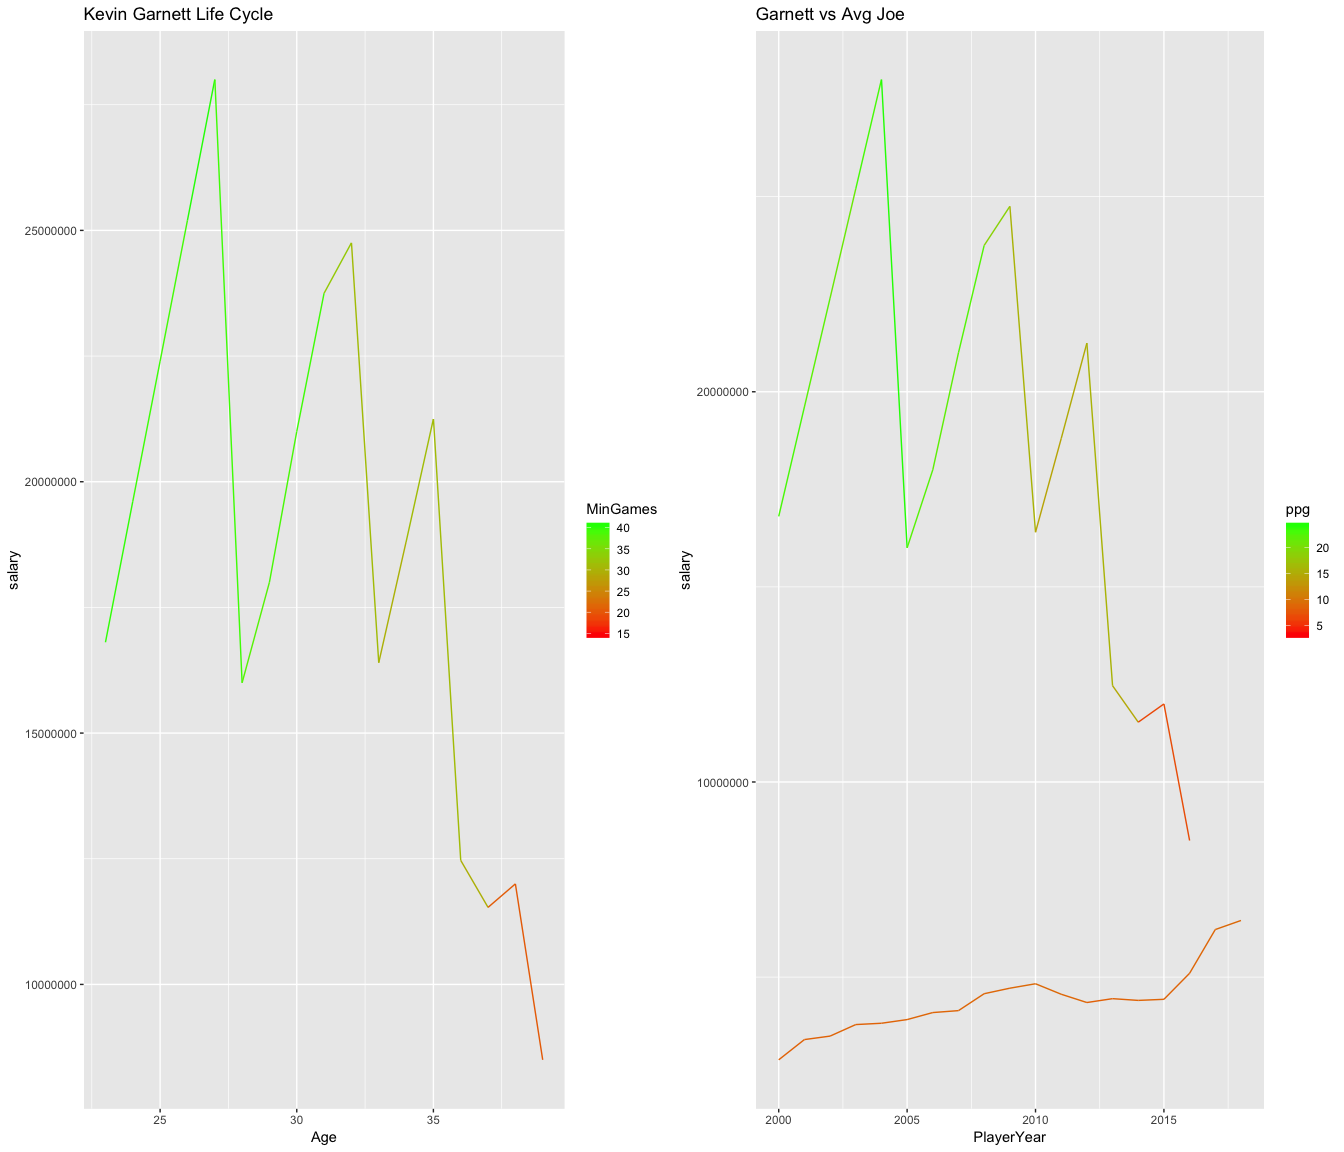
\includegraphics{nba_data_visV4_files/figure-latex/unnamed-chunk-34-1.pdf}

Dirk took pay cuts as well. His production also started to decrease. It
would be interesting to compare height and player life cycle.

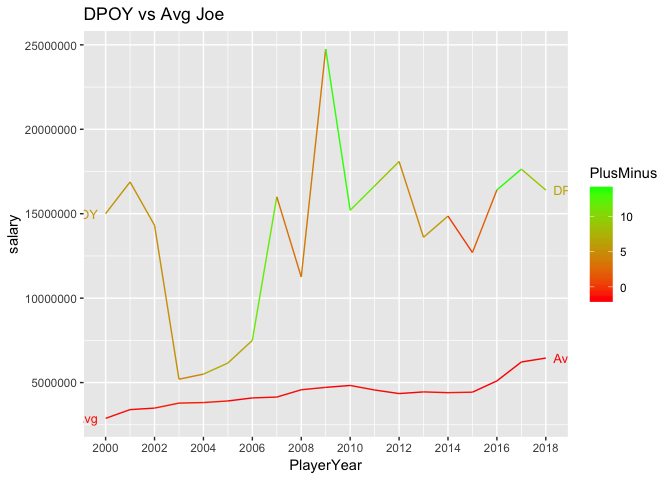
\includegraphics{nba_data_visV4_files/figure-latex/unnamed-chunk-35-1.pdf}

Taller players that make it past year 10 seem to have a longer life
cycle.

\textbf{Stars}

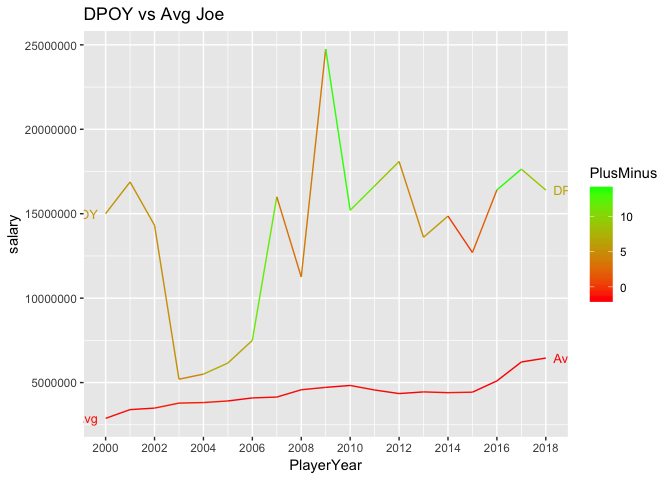
\includegraphics{nba_data_visV4_files/figure-latex/unnamed-chunk-36-1.pdf}

Vince Carters Life cycle goes up in years where it reaches its peak in
his 30s then begins to decrease. Pay goes up because of new contract
deals for NBA players increasing the overall salary cap.

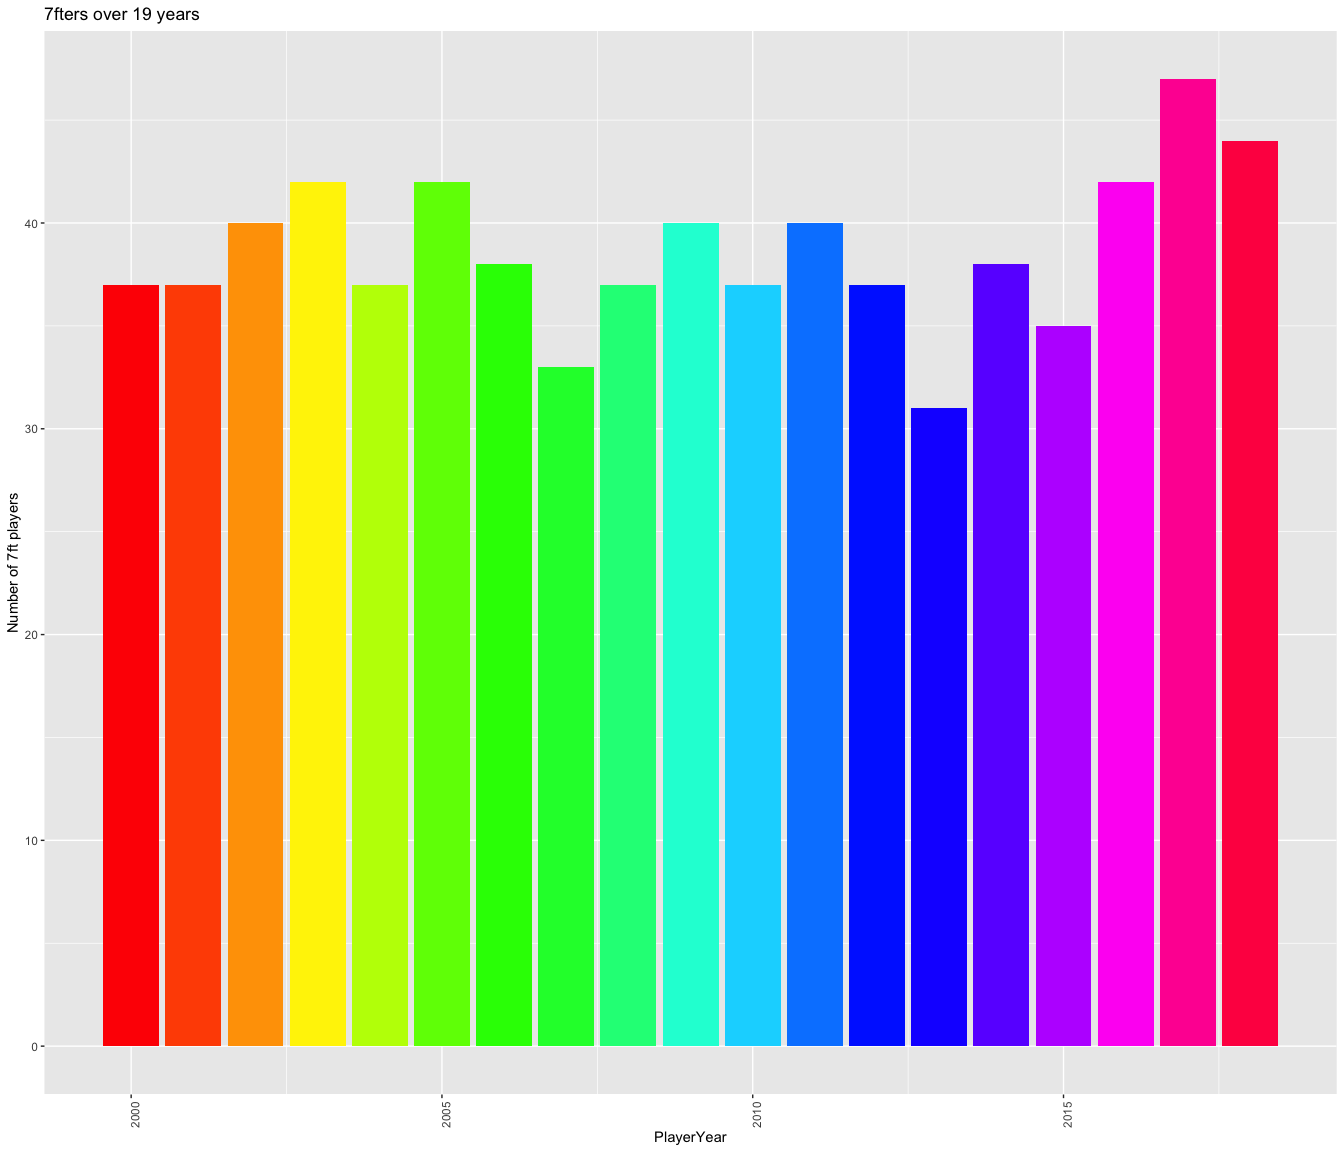
\includegraphics{nba_data_visV4_files/figure-latex/unnamed-chunk-37-1.pdf}

Manu had a decrease in salary pay as he passed 35. But as soon as the
contract money got signed the new TV deal he got paid due to an increase
in salary cap overall.

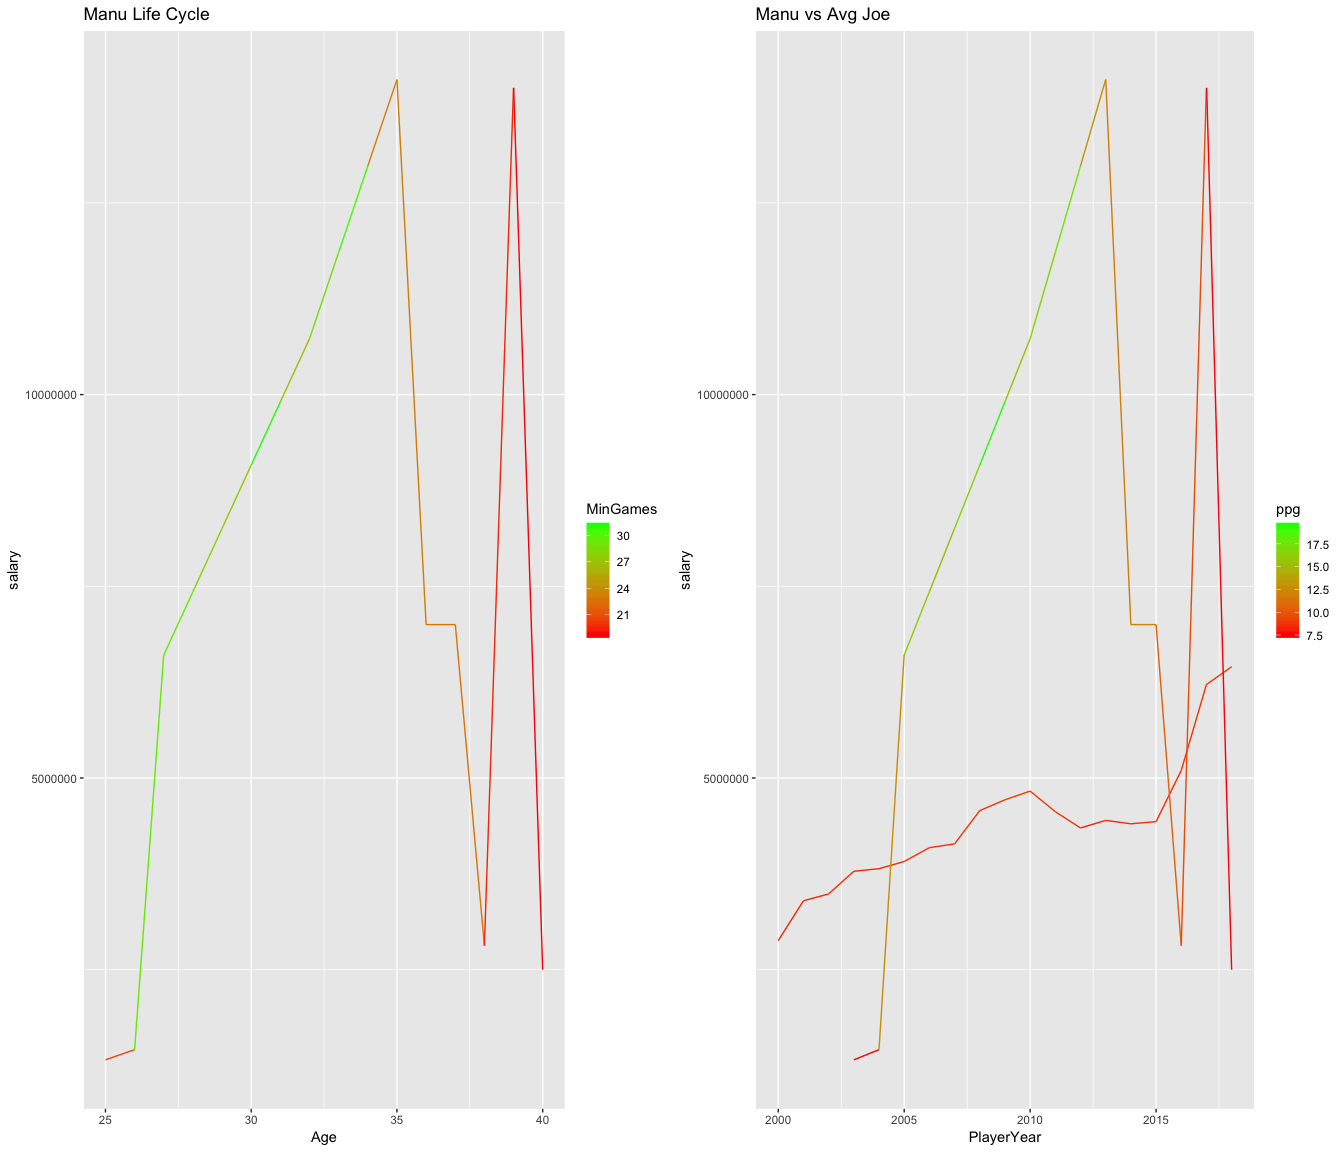
\includegraphics{nba_data_visV4_files/figure-latex/unnamed-chunk-38-1.pdf}

There is no decreasein salary for Melo. However, this player is out of
the league now due to the ineffciency.

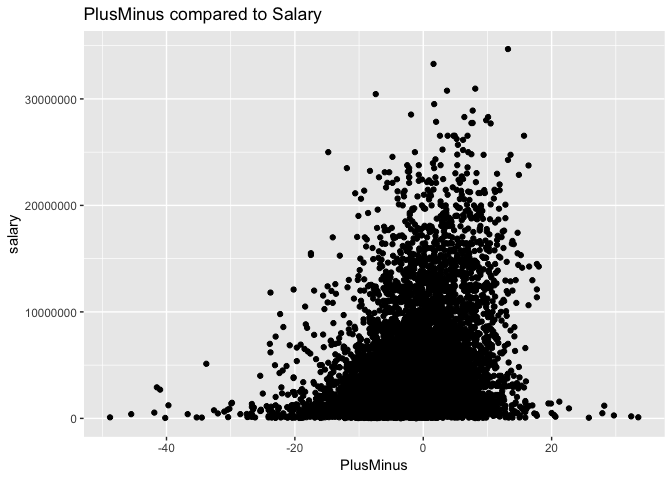
\includegraphics{nba_data_visV4_files/figure-latex/unnamed-chunk-39-1.pdf}

Gasol also had a decrease in salary but the new TV money seems to have
set in a new reference point on how much veterans should be paid.

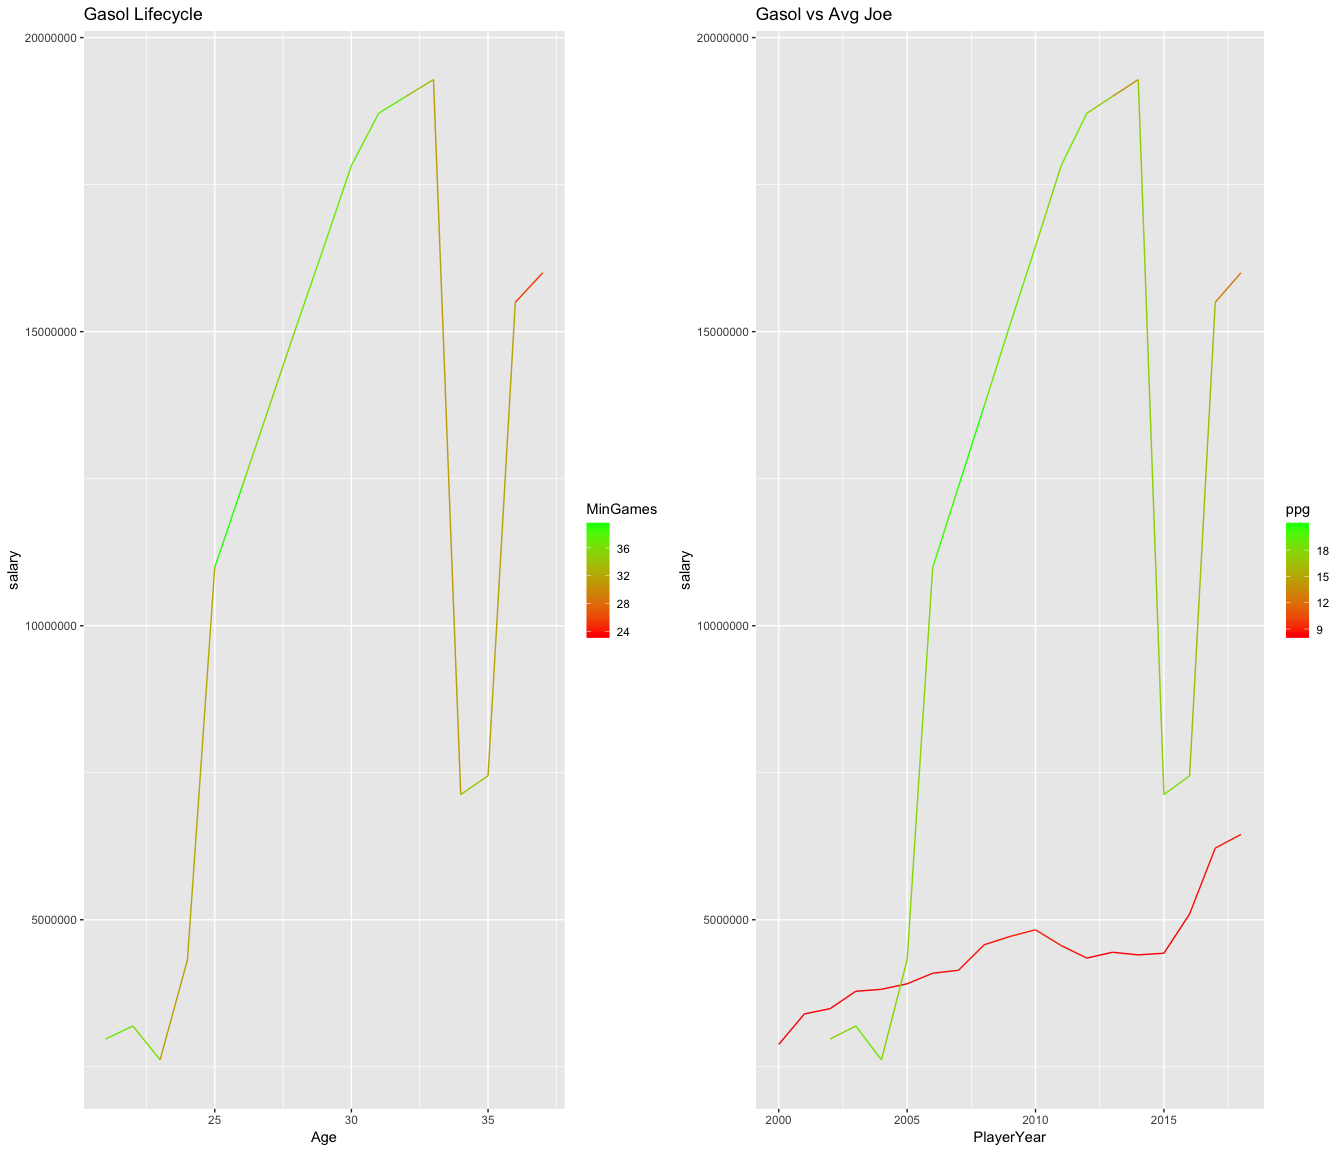
\includegraphics{nba_data_visV4_files/figure-latex/unnamed-chunk-40-1.pdf}

Parkers salary went down but again due to the new TV contract money the
salary did increase back up again even though the player was aging.

RolePlayer
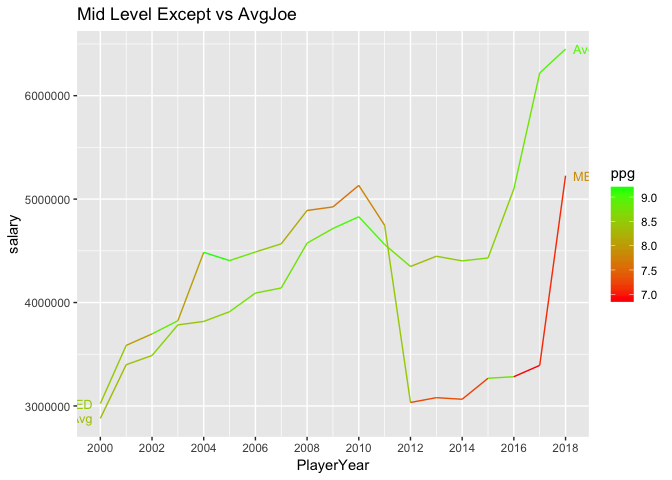
\includegraphics{nba_data_visV4_files/figure-latex/unnamed-chunk-41-1.pdf}

Nene salary decreased. Probably got the veterans minimum with the new
2017 CBA.

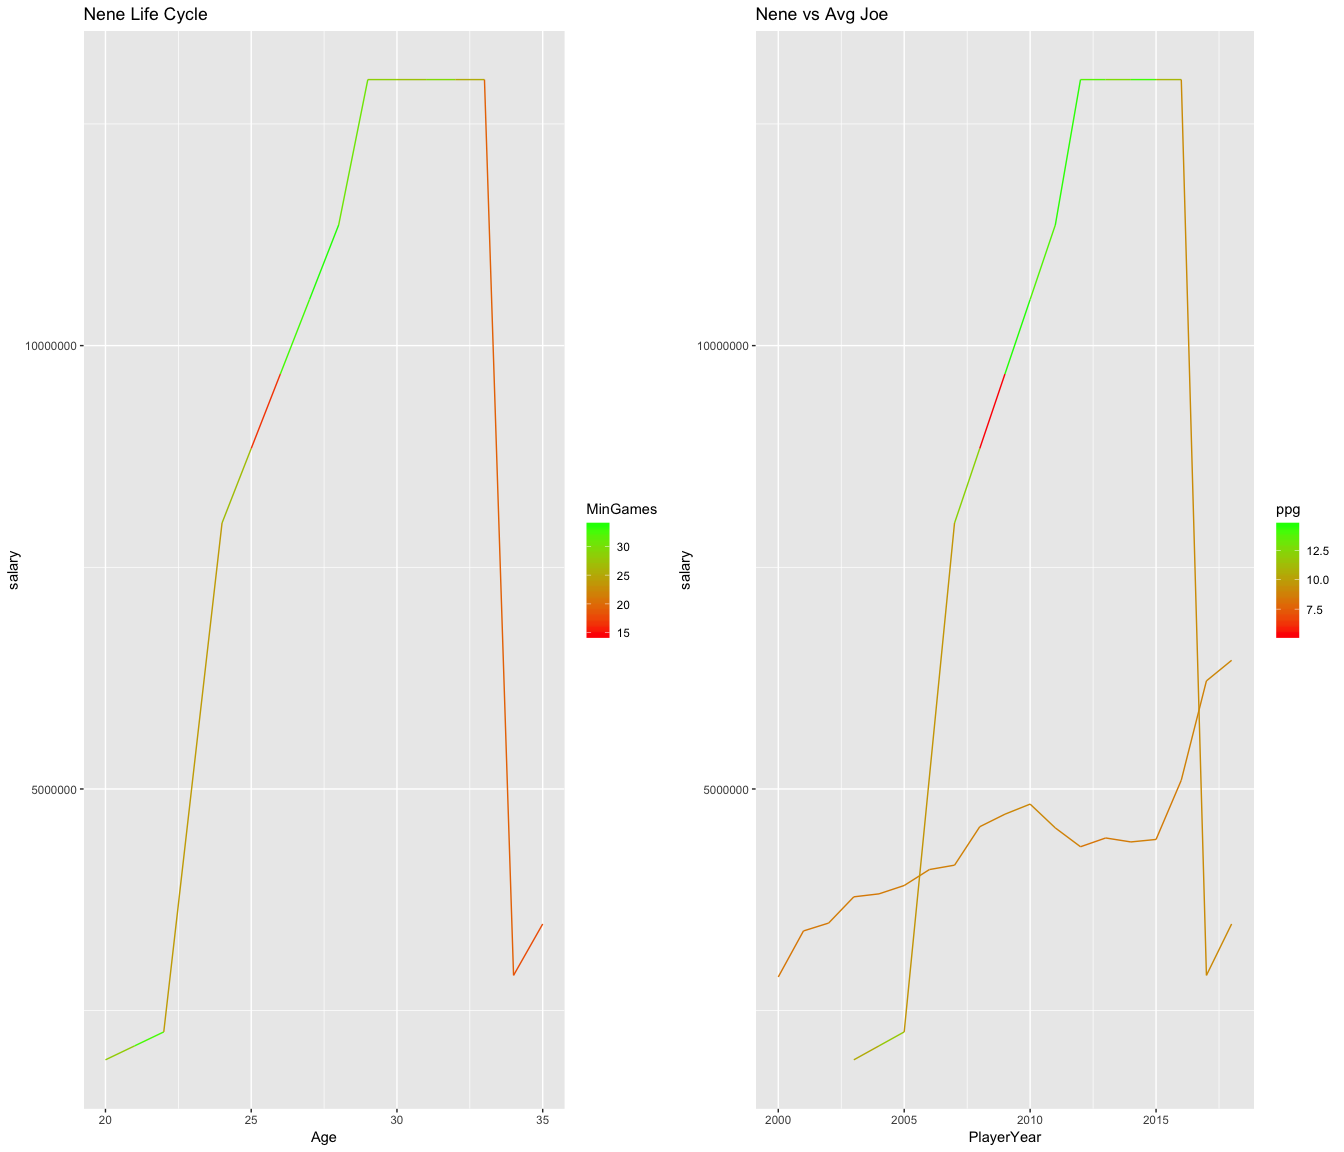
\includegraphics{nba_data_visV4_files/figure-latex/unnamed-chunk-42-1.pdf}

Mike Miller took a pay cut probably to play for a contender.

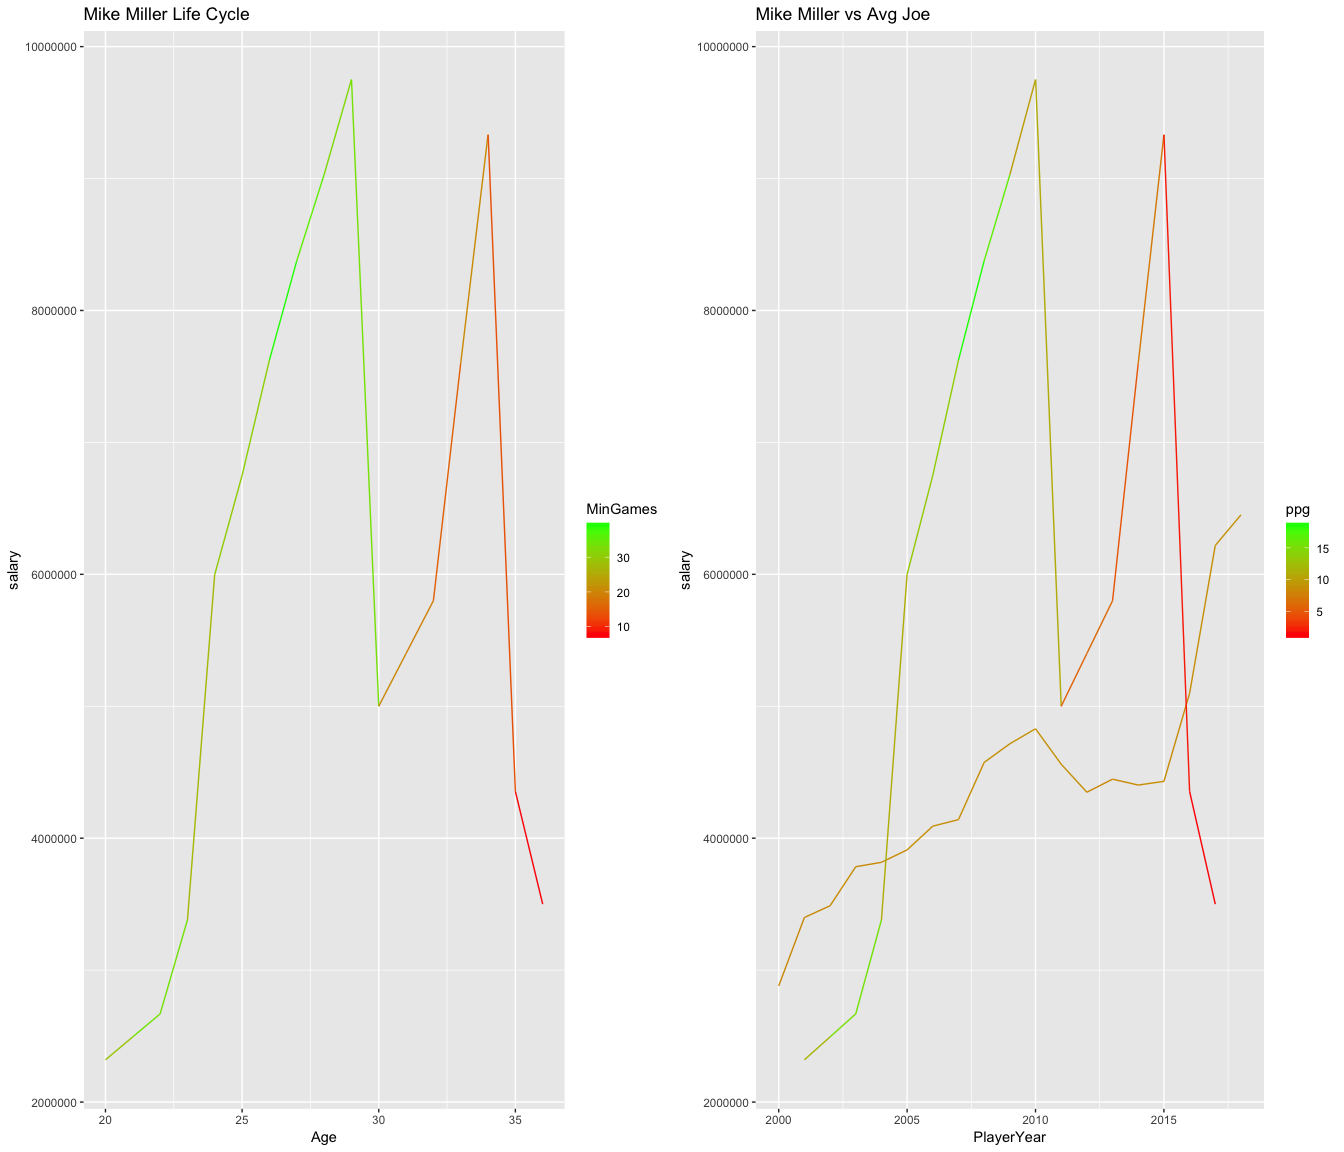
\includegraphics{nba_data_visV4_files/figure-latex/unnamed-chunk-43-1.pdf}

Dunleavy had a pay decrease then a small increase because of the salary
bump overall.

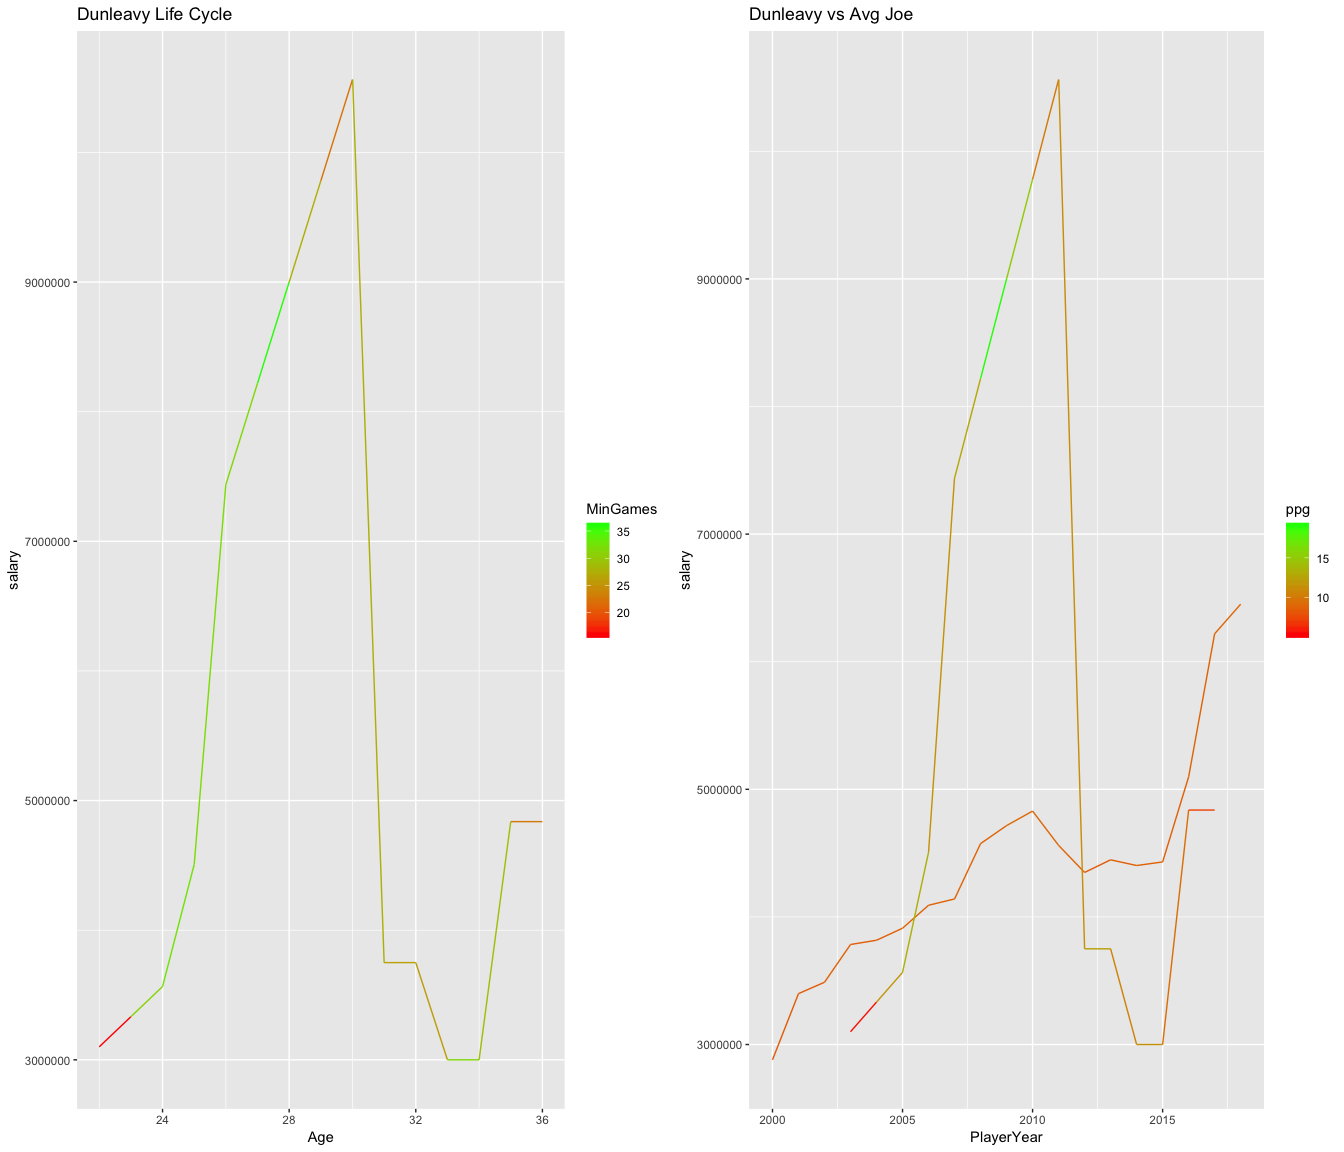
\includegraphics{nba_data_visV4_files/figure-latex/unnamed-chunk-44-1.pdf}

Jamal Crawford got a huge payday after the new TV money after an initial
decrease.

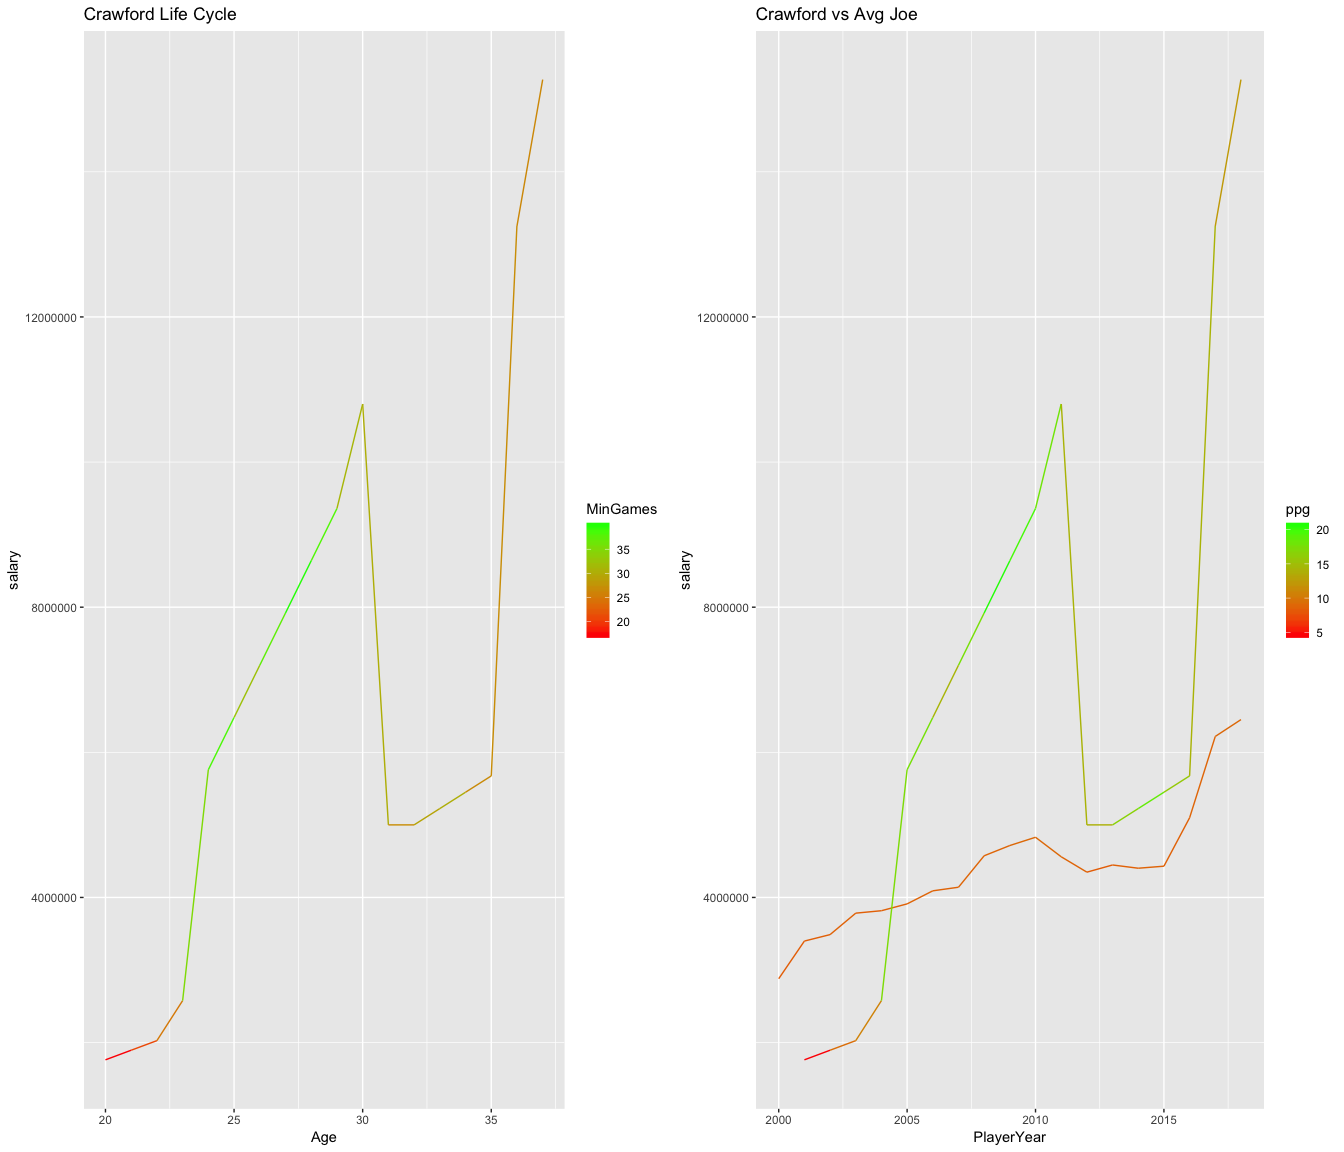
\includegraphics{nba_data_visV4_files/figure-latex/unnamed-chunk-45-1.pdf}

Fisher never made it to the new TV contract money. His salary follows a
normal trend according to his age.

\subsubsection{MVP, DPOY, ROY, MIP, MAX salary trends and MIN salary
trends Mid level exception
trends}\label{mvp-dpoy-roy-mip-max-salary-trends-and-min-salary-trends-mid-level-exception-trends}

\textbf{MVP}

\begin{verbatim}
##      PlayerYear   salary height_cm PlusMinus MinGames  ppg       EFG
## 37         2000 14000000       206       8.9     35.9 25.5 0.5111111
## 776        2001 19285715       216       8.7     39.5 28.7 0.5729167
## 972        2002 11250000       183       5.7     43.7 31.4 0.4226619
## 1243       2003 12072500       214       9.6     39.3 23.3 0.5145349
## 1639       2004 12676125       214      11.4     36.6 22.3 0.5029240
## 2267       2005 16000000       211       2.5     38.1 22.2 0.5030120
## 2772       2006  9625000       191       8.1     35.4 18.8 0.5783582
## 2952       2007 10500000       191      11.1     35.3 18.6 0.6132812
## 3488       2008 16360094       214       9.0     36.0 23.6 0.5087719
## 3741       2009 21262500       198      11.2     36.1 26.8 0.5023923
## 4106       2010 15779912       203      11.1     39.0 29.7 0.5447761
## 4569       2011 14500000       203      10.1     38.8 26.7 0.5425532
## 4859       2012  6993708       191      10.4     35.3 21.8 0.4719101
## 5527       2013 17545000       203      12.4     37.9 26.8 0.6067416
## 6107       2014 19067500       203       7.2     37.7 27.1 0.6107955
## 6413       2015 19997513       206       9.0     33.8 25.4 0.5780347
## 6635       2016 11370786       191      17.7     34.2 30.1 0.6311881
## 7091       2017 12112359       191      17.7     33.4 25.3 0.5765027
## 7785       2018 28299399       191       6.4     36.4 25.4 0.4786730
\end{verbatim}

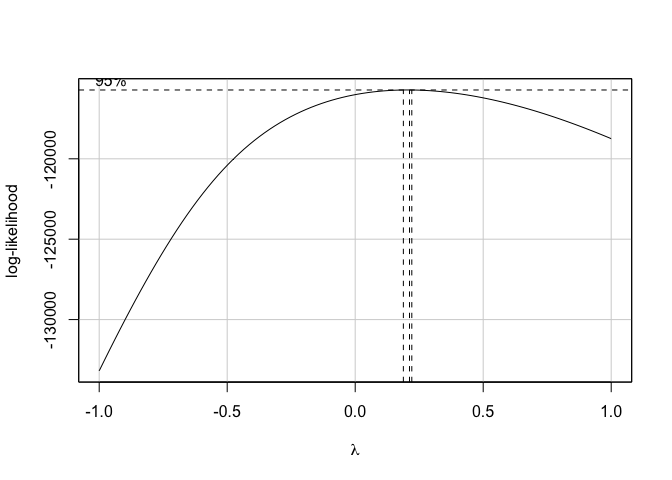
\includegraphics{nba_data_visV4_files/figure-latex/unnamed-chunk-46-1.pdf}

MVPs get more money than the average joe and they should.

\begin{verbatim}
##      PlayerYear   salary height_cm PlusMinus MinGames  ppg       EFG Type
## 370        2000 15004800       208       5.4     34.8 21.7 0.5533333 DPOY
## 542        2001 16880000       208       5.3     23.5 13.6 0.5185185 DPOY
## 884        2002 14315790       219       5.1     36.3 11.5 0.5000000 DPOY
## 1584       2003  5200000       206       4.2     39.4  6.9 0.4833333 DPOY
## 1640       2004  5500000       206       7.2     37.7  9.5 0.4239130 DPOY
## 2279       2005  6157895       201       6.7     41.6 24.6 0.5235294 DPOY
## 2504       2006  7500000       206      11.6     35.2  7.3 0.5087719 DPOY
## 3019       2007 16000000       206       3.0     35.0  6.4 0.4545455 DPOY
## 3440       2008 11250000       211       3.7     34.9  9.1 0.4562500 DPOY
## 3646       2009 24751934       211      13.6     31.1 15.8 0.5307692 DPOY
## 4197       2010 15202590       211      11.8     34.7 18.3 0.6078431 DPOY
## 4679       2011 16647180       211       8.8     37.6 22.9 0.5895522 DPOY
## 4978       2012 18091770       211       4.5     38.3 20.6 0.5746269 DPOY
## 5385       2013 13604188       216       6.1     32.8 10.4 0.6393443 DPOY
## 5849       2014 14860523       216       0.2     33.4 14.6 0.4710744 DPOY
## 6179       2015 12700000       211       2.1     30.6  7.2 0.4375000 DPOY
## 6983       2016 16407500       201      13.8     33.1 21.2 0.5695364 DPOY
## 7278       2017 17638063       201       8.8     33.4 25.5 0.5423729 DPOY
## 7764       2018 16400000       201       6.4     32.7 11.0 0.5170455 DPOY
\end{verbatim}

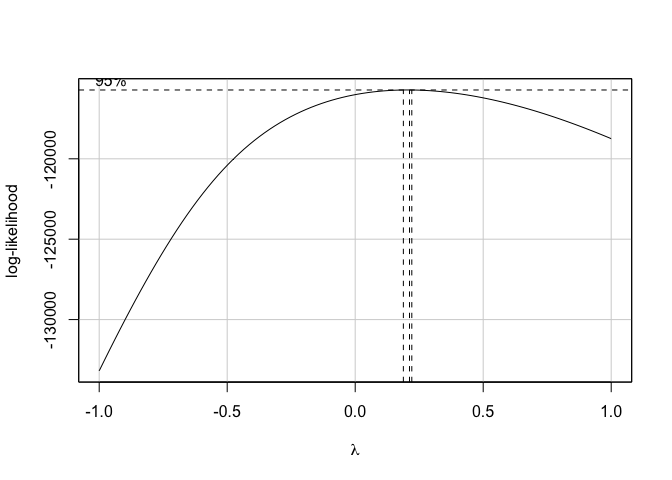
\includegraphics{nba_data_visV4_files/figure-latex/unnamed-chunk-47-1.pdf}

Defensive player of the year doesn't get as much as the MVP but still
more than the average joe.

\begin{verbatim}
##      PlayerYear  salary height_cm PlusMinus MinGames  ppg       EFG
## 412        2000 2267280       201       3.2     38.1 25.7 0.4927536
## 786        2001 3629160       203      -8.0     39.3 20.1 0.4756098
## 827        2002 2494080       203       4.0     33.7 15.2 0.5118110
## 1363       2003 3193680       214      -2.2     36.0 19.0 0.5073529
## 1652       2004 1899720       208      -2.3     36.8 20.6 0.4777070
## 2172       2005 4320360       203       2.2     42.4 27.2 0.5023697
## 2413       2006 4020120       208      -4.2     33.6 13.2 0.4098361
## 3085       2007 3380160       183      -1.0     36.8 17.3 0.4705882
## 3504       2008 2883120       198       0.8     37.7 19.1 0.4873418
## 3686       2009 4484040       206      -8.6     39.0 25.3 0.5079787
## 4046       2010 5184480       191      -0.4     36.8 20.8 0.4943182
## 4742       2011 3880920       198      -4.5     37.0 17.8 0.4329268
## 5123       2012 5731080       208       7.5     36.2 20.7 0.5483871
## 5479       2013 5530080       191      -4.4     34.7 22.5 0.5027624
## 6101       2014 3202920       191       6.0     35.8 20.7 0.5062893
## 6583       2015 2300040       198      -3.6     32.6 14.6 0.4136691
## 6716       2016 5758680       203      -1.0     35.1 20.7 0.4781250
## 7178       2017 5960160       214       0.0     37.0 25.1 0.5777778
## 7861       2018 1312611       196      -2.4     29.9 13.0 0.5476190
\end{verbatim}

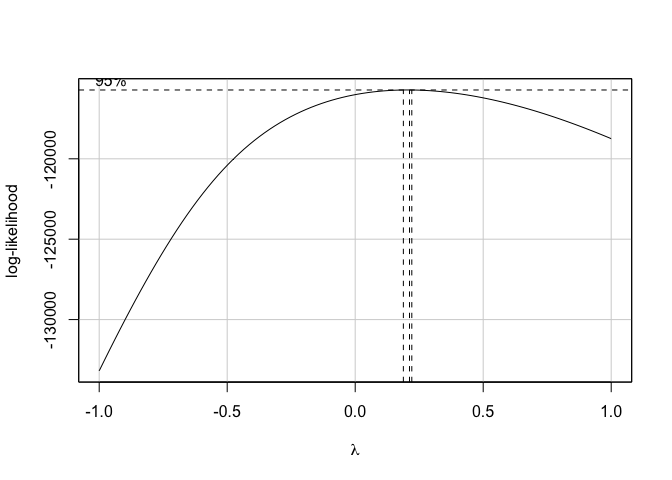
\includegraphics{nba_data_visV4_files/figure-latex/unnamed-chunk-48-1.pdf}

Rookie salary took a dip after the new TV contract deal included in the
2017 CBA. Rookies get paid far less now compared to the average joe.

\begin{verbatim}
##      PlayerYear   salary height_cm PlusMinus MinGames  ppg       EFG
## 154        2000  4125000       186       1.0     31.6 16.2 0.4963235
## 431        2001  9660000       203      -0.3     40.9 20.5 0.4797688
## 1021       2002 10865250       203       5.2     38.3 25.6 0.4832536
## 1498       2003  6900000       211       3.5     37.2 20.8 0.4847561
## 1783       2004  8536000       191      -4.5     37.6 19.6 0.4608434
## 2394       2005  1504272       206      -2.9     34.8 18.9 0.4472050
## 2701       2006  8000000       198       1.3     33.8 13.4 0.5185185
## 2948       2007  1870501       203       5.1     31.1  9.7 0.5512821
## 3497       2008   770610       191       3.1     37.9 20.2 0.5331126
## 4308       2010  9930500       203      -0.1     36.7 24.1 0.4972826
## 4492       2011  2016692       183      -6.6     21.8 10.7 0.4343434
## 5110       2012  4609701       208       0.7     39.0 26.0 0.4948187
## 5360       2013  8700000       208      -5.1     30.9 16.2 0.5144928
## 6095       2014  3282003       206       6.7     36.2 21.7 0.4911765
## 6528       2015  7500000       191      -0.2     33.8 16.3 0.5468750
## 6625       2016 16407500       201      -0.1     36.9 20.9 0.4870130
## 7476       2017  3219579       191       1.0     35.0 23.0 0.5472222
## 7860       2018 22471911       211       3.1     36.7 26.9 0.5454545
\end{verbatim}

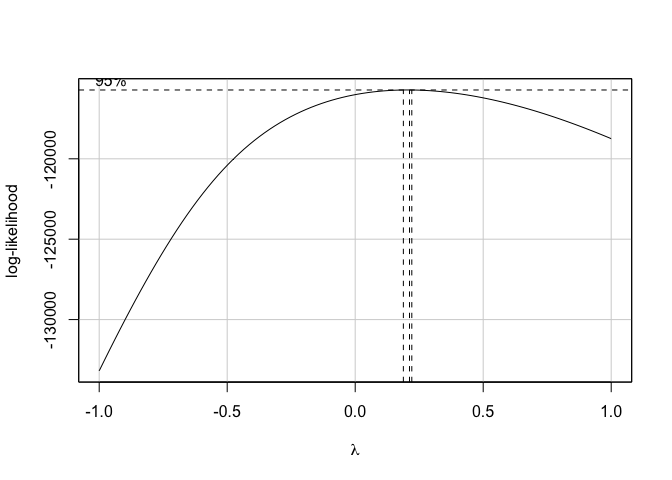
\includegraphics{nba_data_visV4_files/figure-latex/unnamed-chunk-49-1.pdf}

MIP tends to get more money than the average Joe. Some years dipping
below. Probably getting a pay increase after winning the award. Would be
interesting to look at the trend.

\textbf{MAX}

\begin{verbatim}
##               name PlayerYear   salary height_cm PlusMinus MinGames  ppg
## 7548 Stephen Curry       2018 34682550       191      13.2     32.0 26.4
## 90    LeBron James       2017 30963450       203       8.1     37.8 26.4
## 252    Kobe Bryant       2016 25000000       198     -14.8     28.2 17.6
## 15     Kobe Bryant       2015 23500000       198     -11.9     34.5 22.3
## 143    Kobe Bryant       2014 30453000       198      -7.4     29.5 13.8
## 9      Kobe Bryant       2013 27849000       198       2.0     38.6 27.3
## 219    Kobe Bryant       2012 25244493       198       3.0     38.5 27.9
## 315    Kobe Bryant       2011 24806250       198       7.5     33.9 25.3
## 244  Tracy McGrady       2010 23239562       203      -8.3     22.4  8.2
## 13   Kevin Garnett       2009 24751934       211      13.6     31.1 15.8
##            EFG
## 7548 0.6213018
## 90   0.5906593
## 252  0.4142012
## 15   0.4093137
## 143  0.4467213
## 9    0.5073529
## 219  0.4630435
## 315  0.4850000
## 244  0.4166667
## 13   0.5307692
\end{verbatim}

\includegraphics{nba_data_visV4_files/figure-latex/unnamed-chunk-50-1.pdf}

Max player obviously each year gets more for their production everyyear
over the average joe.

\textbf{Minimum Salary}

To find which players qualified for the min salary. We took the salary
for players that at least played 1 year in the NBA.

\begin{verbatim}
##    PlayerYear   salary height_cm PlusMinus MinGames      ppg       EFG
## 1        2018 592275.9  197.6429 -3.940179 14.71339 5.062500 0.4733439
## 2        2017 526671.2  198.3390 -3.752542 13.66780 4.613559 0.4810943
## 3        2016 486266.1  200.3704 -5.225926 13.48889 4.598148 0.4586663
## 4        2015 472604.7  199.0000 -5.264179 13.94627 4.628358 0.4556341
## 5        2014 496228.7  199.6533 -1.742667 13.88667 4.420000 0.4600698
## 6        2013 510376.4  198.9286 -3.623214 12.72321 4.033929 0.4647649
## 7        2012 464745.3  199.2982 -5.182456 12.74035 4.043860 0.4547385
## 8        2011 464942.7  199.0000 -4.469767 13.21163 4.683721 0.4710174
## 9        2010 454989.9  199.2927 -4.160976 14.30976 5.053659 0.4746463
## 10       2009 511001.2  198.8857 -4.068571 13.80857 4.260000 0.4809072
\end{verbatim}

\includegraphics{nba_data_visV4_files/figure-latex/unnamed-chunk-51-1.pdf}

Min player of course is under the average joe player salary.

\textbf{Mid Level Exception } To see if a team could possibily sign a
player went with 25 percent over and under the mid level exception
everyyear. Also, did not want to have a player drafted that year as well
as no player under 23 for that year.

\begin{verbatim}
##                   name  ppg PlusMinus MinGames Games PlayerYear
## 6255     Klay Thompson 21.7      15.3     31.9    77       2015
## 6317    Damian Lillard 21.0       5.3     35.7    82       2015
## 6348       Danny Green 11.7       9.7     28.5    81       2015
## 6379 Marreese Speights 10.4       7.7     15.9    76       2015
## 6388       Matt Barnes 10.1      11.7     29.9    76       2015
## 6406    Anthony Morrow 10.7       5.5     24.4    74       2015
## 5821   Marco Belinelli 11.4       6.5     25.2    80       2014
## 5468      Vince Carter 13.4       5.5     25.8    81       2013
## 5529         Ty Lawson 16.7       5.4     34.4    73       2013
## 5612          JR Smith 18.1       5.7     33.5    80       2013
\end{verbatim}

These are notable mid level exception players that fell into the
category. Except for Damian Lilard and Klay most of these players could
have possibly be signed to a mid level exception if they were free
agents due to bad team management.

\begin{verbatim}
##    PlayerYear  salary height_cm  PlusMinus MinGames      ppg       EFG
## 1        2018 5226548  199.8919 -1.4594595 19.97838 7.862162 0.5142168
## 2        2017 3392485  199.9000 -1.4300000 18.22250 7.077500 0.5026139
## 3        2016 3282897  201.0238 -1.2666667 18.58095 6.902381 0.4972249
## 4        2015 3267768  199.6735 -0.2469388 21.51633 8.748980 0.4935115
## 5        2014 3064909  202.5106 -0.6297872 19.58936 7.225532 0.5069429
## 6        2013 3080277  200.3958 -0.9916667 19.80833 7.329167 0.4928712
## 7        2012 3033485  202.2500 -1.4192308 21.43654 7.290385 0.4944566
## 8        2011 4746809  200.3542 -1.4395833 22.56667 8.477083 0.4938972
## 9        2010 5132612  200.6364 -0.3545455 22.12182 7.790909 0.4983103
## 10       2009 4924562  201.4000 -0.0320000 22.65800 7.588000 0.4923068
\end{verbatim}

\includegraphics{nba_data_visV4_files/figure-latex/unnamed-chunk-53-1.pdf}

Mid level player used to get paid more but probably because of the
previous CBA and building superteams they cut the amount so good maxed
out teams cannot sign a good player with a huge mid level exception
salary.


\end{document}
